% !TEX root = ../../../../temp_manuscript.tex

\chapter[DeepDicomSort: An automatic sorting algorithm for brain magnetic resonance imaging data][DeepDicomSort]{DeepDicomSort: An automatic sorting algorithm for brain magnetic resonance imaging data}\label{chap:DDS}
\begin{ChapterAbstract}
With the increasing size of \glspl{ds} used in medical imaging research, the need for automated data curation is arising.
One important data curation task is the structured organization of a \gls{ds} for preserving integrity and ensuring reusability.
Therefore, we investigated whether this data organization step can be automated.
To this end, we designed a \gls{CNN} that automatically recognizes eight different brain \gls{MRI} \glspl{type} based on visual appearance.
Thus, our method is unaffected by inconsistent or missing \gls{scan} metadata.
It can recognize \gls{T1}, \gls{T1C}, \gls{T2}, \gls{PD}, \gls{FLAIR}, \gls{DWI}, \gls{DSC} \glspl{scan} and derived maps (e.g. \acrlong{ADC} and cerebral blood flow).
In a first experiment, we used \glspl{scan} of \glspl{sub} with brain \glspl{tumor}: \num{11065} \glspl{scan} of \num{719} \glspl{sub} for training, and \num{2369} \glspl{scan} of \num{192} \glspl{sub} for testing.
The \gls{CNN} achieved an overall accuracy of \per{98.7}.
In a second experiment, we trained the \gls{CNN} on all \num{13434} \glspl{scan} from the first experiment and tested it on \num{7227} \glspl{scan} of \num{1318} Alzheimer's \glspl{sub}.
Here, the \gls{CNN} achieved an overall accuracy of \per{98.5}.
In conclusion, our method can accurately predict \gls{type}, and can quickly and automatically sort a brain \gls{MRI} \gls{ds} virtually without the need for manual verification.
In this way, our method can assist with properly organizing a \gls{ds}, which maximizes the shareability and integrity of the data.

\publishedas{vandervoort2020deepdicomsort}
\end{ChapterAbstract}
\setcellgapes{5pt}


% To not show acronyms
\glsunset{sub}
\glsunset{ses}
\glsunset{scan}
\glsunset{type}
\glsunset{slice}
\glsunset{ds}
\glsunset{sample}
\glsunset{class}
\glsunset{HC}
\glsunset{site}
\glsunset{NTTS}
\glsunset{BTtrain}
\glsunset{BTtest}
\glsunset{BTset}
\glsunset{TCGAGBM}
\glsunset{TCGALGG}
\glsunset{LGG1p19q}
\glsunset{BTP}
\glsunset{}

\section{Introduction}

With the rising popularity of machine learning, deep learning, and automatic pipelines in the medical imaging field, the demand for large \glspl{ds} is increasing.
To satisfy this hunger for data, the amount of imaging data collected at healthcare institutes keeps growing, as is the amount of data that is shared in public repositories \autocite{greenspan2016deep, lundervold2019overview}.
However, this increase in available data also means that proper data curation, the management of data throughout its life cycle, is needed to keep the data manageable and workable \autocite{prevedello2019challenges, vanooijen2019quality}.
One essential data curation step is organizing a \gls{ds} such that it can easily be used and reused.
Properly organizing the \gls{ds} maximizes the shareability and preserves the full integrity of the \gls{ds}, ensuring repeatability of an experiment and reuse of the \gls{ds} in other experiments.

Unfortunately, the organization of medical imaging data is not standardized, and the format in which a \gls{ds} is provided often differs between sources \autocite{lambin2017radiomics, vanooijen2019quality}.
Efforts such as the \gls{BIDS} \autocite{gorgolewski2016brain} propose a standardized data structure, to which some public data repositories adhere (e.g. OpenNeuro \autocite{gorgolewski2017openneuro}, \gls{ABIDE} \autocite{dimartino2017enhancing} and \gls{OASIS} \autocite{lamontagne2018oasis}).
However, other repositories do not conform to this standard (e.g. \gls{TCIA} \autocite{clark2013cancer}, \gls{ADNI}, and \gls{PPMI} \autocite{marek2018parkinson}).
Furthermore, similar to some prospectively collected research data, retrospectively collected data from clinical practice usually do not follow a standardized format either \autocite{vanooijen2019quality}.
Thus, the challenge of structuring a \gls{ds}, either into a \gls{BIDS} compliant \gls{ds} or a different format, remains.

When using a medical imaging \gls{ds} in a research project, one needs to select the \glspl{type} that are relevant to the research question \autocite{montagnon2020deep, lambin2017radiomics}.
Thus, it is essential to identify the \gls{type} of each \gls{scan} when sorting a medical imaging \gls{ds}.
Different data sources do not use consistent naming conventions in the metadata of a \gls{scan} (e.g. the series description), which complicates the automatic identification of the \gls{type} \autocite{vanooijen2019quality, wang2011automated}.
Moreover, in some cases, this metadata is not consistently stored (e.g. contrast administration \autocite{hirsch2015we}) and might even be partially or entirely missing, as can be the case for anonymized data \autocite{moore2015identification}.
As a result, the sorting is frequently done manually, by looking at each \gls{scan} and labeling it according to the perceived \gls{type}.
This manual labeling can be a very time-consuming task, which hampers scientific progress; thus, it is highly desirable to automate this step of the data curation pipeline.
Similar arguments concerning the complexity of medical imaging data and the importance of data structuring also motivated the creation of the \gls{BIDS} standard \autocite{gorgolewski2016brain}.

Previous research has focused on modality recognition \autocite{dimitrovski2015improved,yu2015modality,arias2016medical}, as well as on distinguishing different modalities of \gls{MRI} \glspl{scan} \autocite{srinivas2014medical,remedios2018classifying}.
Only one of these studies \autocite{remedios2018classifying} considered the prediction of the \gls{type} of \gls{MRI} \glspl{scan}, who predicted \num{4} \glspl{type}, namely \gls{T1}, \gls{T1C}, fluid-attenuated inversion recovery (FLAIR) and \gls{T2} \glspl{scan}.
However, with the increasing popularity of multi-parametric \gls{MRI} in machine learning algorithms and automatic pipelines \autocite{li2017deep,akkus2017predicting,nie20163d,pereira2015deep}, the need to recognize more \glspl{type} is arising.

In this research, we propose a method, called \gls{DDS}, that recognizes eight different \glspl{type} of brain \gls{MRI} \glspl{scan}, and facilitates sorting into a structured format.
\gls{DDS} is a pipeline consisting of a pre-processing step to prepare \glspl{scan} as inputs for a \gls{CNN}, a \gls{type} recognition step using a \gls{CNN}, and a post-processing step to sort the identified \glspl{type} into a structured format.
Our method identifies \gls{T1}, \gls{T1C}, \gls{T2}, \gls{PD}, \gls{FLAIR}, \gls{DWI} (including trace/isotropic images), \gls{DSC} \glspl{scan}, and diffusion-weighted and perfusion-weighted derived maps (including, for example, \gls{ADC}, fractional anisotropy, and relative cerebral blood flow).
Once the \glspl{type} have been identified, \gls{DDS} can organize the \gls{ds} into a structured, user-defined layout or turn the \gls{ds} into a \gls{BIDS} compliant \gls{ds}.
We made all our source code, including code for the pre-processing and post-processing, and pre-trained models publicly available, to facilitate reuse by the community\footnote{\url{https://github.com/Svdvoort/DeepDicomSort}}.


\section{Materials \& Methods}
\subsection{Terminology}

Since the exact meaning of specific terms can differ depending on one's background, we have provided an overview of the terminology as it is used in this paper in \cref{tab:terminology}.
We have tried to adhere to the terminology used by \gls{BIDS} as much as possible, and have provided the equivalent \gls{BIDS} terminology in \cref{tab:terminology} as well.
We differ from the \gls{BIDS} terminology regarding two terms: \gls{scan} and \gls{type}.
\Gls{type} is referred to as modality in \gls{BIDS}, but to avoid confusion with the more common use of modality to indicate different types of equipment (e.g. \gls{MRI} and \gls{CT}), we instead use \gls{type}.
\Gls{scan} is used instead of \say{data acquisition} or \say{run} as used in \gls{BIDS}, to be more in line with common terminology and to avoid confusion with other types of data acquisition.
We define a structured \gls{ds} as a \gls{ds} where all the data for the different \glspl{sub} and \glspl{scan} is provided in the same way.
For example, a folder structure with a folder for each \gls{sub}, \gls{ses} and \gls{scan} with a consistent naming format for the different folders and \glspl{type}.
A standardized \gls{ds} is a \gls{ds} where the data has been structured according to a specific, public standard, for example \gls{BIDS}.


\begin{table}[htbp]
  \centering

  \begin{tabular}{L{1.5cm}L{3cm}L{6cm}}
  \toprule
  \textbf{Term} & \textbf{\gls{BIDS} term} & \textbf{Meaning}\\
  \midrule
  Modality & Modality & Type of technique used to acquire a \gls{scan} (e.g. \gls{MRI}, \gls{CT})\\
  \\
  \Gls{sub} & Subject & A person participating in a study\\
  \\
  \Gls{site} & Site & Institute at which a \gls{scan} of the \gls{sub} has been acquired\\
  \\
  \Gls{ses} & Session & A single visit of a \gls{sub} to a \gls{site} in which one or more \glspl{scan} have been acquired\\
  \\
  \Gls{scan} & Data acquisition/run & A single 3D image that has been acquired of a \gls{sub} in a \gls{ses}\\
  \\
  \Gls{slice} & N/A & A single 2D cross-section that has been extracted from a \gls{scan}\\
  \\
  \Gls{type} & Modality & Specific visual appearance category of a \gls{scan} (e.g. \gls{T1}, \gls{T2})\\
  \\
  \Gls{sample} & N/A & A single input for the \gls{CNN}\\
  \\
  \Gls{class} & N/A & An output category of the \gls{CNN}\\
  \\
  \acrshort{DICOM} & \acrshort{DICOM} & A data format used to store medical imaging data. In addition to the imaging data, \acrshort{DICOM} files can also store metadata about the scanner equipment, the specific imaging protocol and clinical information.\\
  \\
  \acrshort{NIFTI} & \acrshort{NIFTI} & A data format used to store (neuro) medical imaging data.\\
  \bottomrule
  \end{tabular}
  \caption{Overview of terminology used in this paper, the corresponding \gls{BIDS} terminology and meaning of each term}\label{tab:terminology}
\end{table}



\subsection{Data}

An extensive collection of data from multiple different sources was used to construct our method and evaluate its performance.
We used \gls{MRI} \glspl{scan} of \glspl{sub} with brain \glspl{tumor}, as well as \glspl{scan} of \glspl{sub} without brain \glspl{tumor}.

To ensure sufficient heterogeneity in our \gls{ds}, we included \glspl{scan} from multiple different sources, and we only excluded \glspl{scan} if their \gls{type} did not fall into one of the eight categories that we aimed at predicting with our method.
Thus, no \glspl{scan} were excluded based on other criteria such as low image quality, the occurrence of imaging artifacts, scanner settings, or disease state of the \gls{sub}.

\subsubsection{\Acrlong{BTset}}
Our method was initially developed and subsequently tested on brain \gls{MRI} \glspl{scan} of \glspl{sub} with brain \glspl{tumor}.
\Glspl{scan} of \glspl{sub} with brain \glspl{tumor} were used because the brain \gls{tumor} imaging protocols used to acquire these \glspl{scan} usually span a wide array of \glspl{type}, including pre-contrast and post-contrast \glspl{scan}.
The \gls{BTset} consisted of a train set and an independent test set, which in total included data from \num{11} different sources.
The \glspl{sub} were distributed among the \gls{BTtrain} and \gls{BTtest} before starting any experiments, and the data was divided such that the distribution of the \glspl{type} was similar in the train set and the test set.
We chose to put all \glspl{sub} that originated from the same \gls{ds} in either the train set or test set to test the generalizability of our algorithm.
Thus, all \glspl{scan} of a \gls{sub} were either all in the \gls{BTtrain} or all in the \gls{BTtest}, and no data leak could take place, precluding an overly optimistic estimation of the performance of our method.
In this way, a good performance of our method on the test set could not be the result of the algorithm having learned features that are specific to a particular \gls{site} or scanner.

The \gls{BTtrain} contained \num{11065} \glspl{scan} of \num{1347} different \glspl{ses} from \num{719} \glspl{sub}.
These \glspl{scan} were included from the \gls{BTP} \autocite{schmainda2018radiology}, \gls{IVY} \autocite{nameeta2016radiology}, \gls{LGG1p19q} \autocite{bradley2017radiology,akkus2017predicting}, \gls{TCGAGBM} \autocite{scarpace2016radiology} and \gls{TCGALGG} \autocite{pedano2016radiology} collections from \gls{TCIA} \autocite{clark2013cancer}.
Two \glspl{ds} from \gls{USIGT} \autocite{fyllingen2016glioblastoma,xiao2017retrospective} were also included in the \gls{BTtrain}.
In total, the data originated from \num{17} different \glspl{site}, and the \glspl{scan} were acquired on at least \num{29} different scanner models from \num{4} different vendors (GE, Hitachi, Philips, and Siemens).

The \gls{BTtest} contained \num{2369} \glspl{scan} of \num{302} different \glspl{ses} from \num{192} \glspl{sub}.
These \glspl{scan} were included from the \gls{BITE} \gls{ds} \autocite{mercier2012online} as well as the \gls{CPTAC} \autocite*{cptac2018radiology}, \gls{REMBRANDT} \autocite{scarpace2015radiology}, and \gls{RIDER} \autocite{barboriak2015radiology} collections from the \gls{TCIA}.
In total, the data originated from \num{8} different \glspl{site}, and the \glspl{scan} were acquired on at least \num{15} different scanner models from \num{4} different vendors (GE, Philips, Siemens, and Toshiba).

For some \glspl{scan}, the scanner type was not available in the \gls{DICOM} tags (\gls{DICOM} tag (0008, 1090)); thus, the data variation in the number of scanners could be even larger.

All \glspl{sub} included in the \gls{BTset} had a (pre-operative or post-operative) brain \gls{tumor}.
The \glspl{scan} in the \glspl{ds} were manually sorted, and \gls{T1}, \gls{T1C}, \gls{T2}, \gls{PD}, \gls{FLAIR}, \gls{DWI}, \gls{DSC}, and derived images were identified.
The different types of derived images were combined into a single category, as the derivation of these images is often inconsistent among scanners and vendors, and thus these images need to be rederived from the raw data (e.g. the original \gls{DWI} or \gls{DSC} \gls{scan}).

The details of the \gls{BTtrain} and \gls{BTtest} are presented in \cref{tab:data_tumor}.
An example of the eight \glspl{type} for a single \gls{sub} from the \gls{BTtest} can be seen in \cref{fig:seq_examples}.

\begin{table}[htbp]
    \centering

    \newlength\scantablewidth
    \setlength\scantablewidth{0.6cm}
    \newlength\datasetsep
    \setlength\datasetsep{20pt}
    \newlength\totaldata
    \setlength\totaldata{0.8cm}

    \setlength{\tabcolsep}{3pt}

    \begin{tabular}{L{1.78cm}S[table-format=4.0]S[table-format=4.0]S[table-format=4.0]S[table-format=4.0]S[table-format=5.0]C{\datasetsep}S[table-format=4.0]S[table-format=4.0]S[table-format=4.0]S[table-format=4.0]S[table-format=4.0]}
    \toprule
    &\multicolumn{5}{c}{\textbf{\Acrlong{BTtrain}}}&&\multicolumn{5}{c}{\textbf{\Acrlong{BTtest}}}\\
    \cmidrule(l){2-6}\cmidrule(l){8-12}
    {\textbf{\Gls{type}}} & {Ax} & {Cor} & {Sag} & {3D} & {Total}&& {Ax} & {Cor} & {Sag} & {3D} & {Total}\\
    \midrule
     \acrshort{T1}       & 580  & 14   & 872  & 454  & 1920  & & 206  & 2    & 202  & 26   & 436\\
     \acrshort{T1C}      & 964  & 526  & 298  & 1040 & 2828  & & 208  & 133  & 97   & 172  & 610\\
     \acrshort{T2}       & 1151 & 411  & 23   & 31   & 1616  & & 232  & 46   & 16   & 1    & 295\\
     \acrshort{PD}       & 413  & 40   & 0    & 0    & 453   & & 145  & 36   & 0    & 0    & 181\\
     \acrshort{FLAIR}    & 991  & 39   & 4    & 50   & 1084  & & 221  & 3    & 0    & 32   & 256\\
     \acrshort{DWI}      & 1359 & 0    & 0    & 0    & 1359  & & 347  & 0    & 0    & 0    & 347\\
     \acrshort{DSC}      & 669  & 0    & 0    & 0    & 669   & & 87   & 0    & 0    & 0    & 87\\
     Derived        & 1136 & 0    & 0    & 0    & 1136  & & 157  & 0    & 0    & 0    & 157\\
     \midrule
     \textbf{Total} & 7263 & 1030 & 1197 & 1575 & 11065 & & 1603 & 220  & 315  & 231  & 2369\\
     \bottomrule
    \end{tabular}
    \caption{Overview of data in the \gls{BTset}. The number of \glspl{scan} for each \gls{type} and the different spatial orientations (axial, coronal, sagittal, and 3D) are specified}\label{tab:data_tumor}
\end{table}

\begin{figure}
\centering

\newlength{\figexamplewidth}
\setlength{\figexamplewidth}{0.22\textwidth}

\begin{subfigure}[t]{\figexamplewidth}
    \centering
    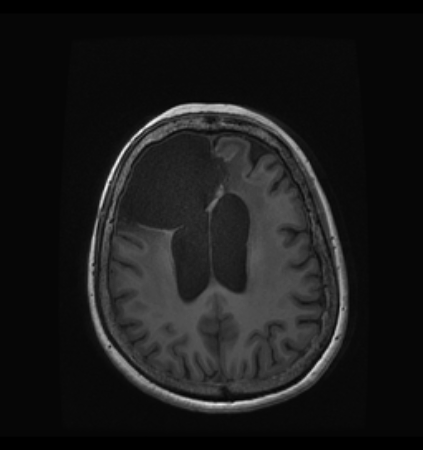
\includegraphics[width=\textwidth]{Figures/T1}
    \caption{\gls{T1}}\label{fig:T1}
\end{subfigure}
\begin{subfigure}[t]{\figexamplewidth}
    \centering
    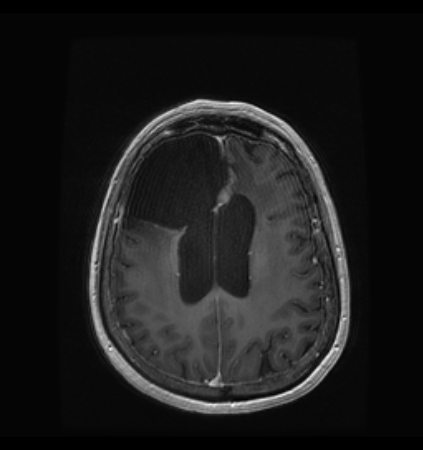
\includegraphics[width=\textwidth]{Figures/T1GD}
    \caption{\gls{T1C}}\label{fig:T1GD}
\end{subfigure}
\begin{subfigure}[t]{\figexamplewidth}
    \centering
    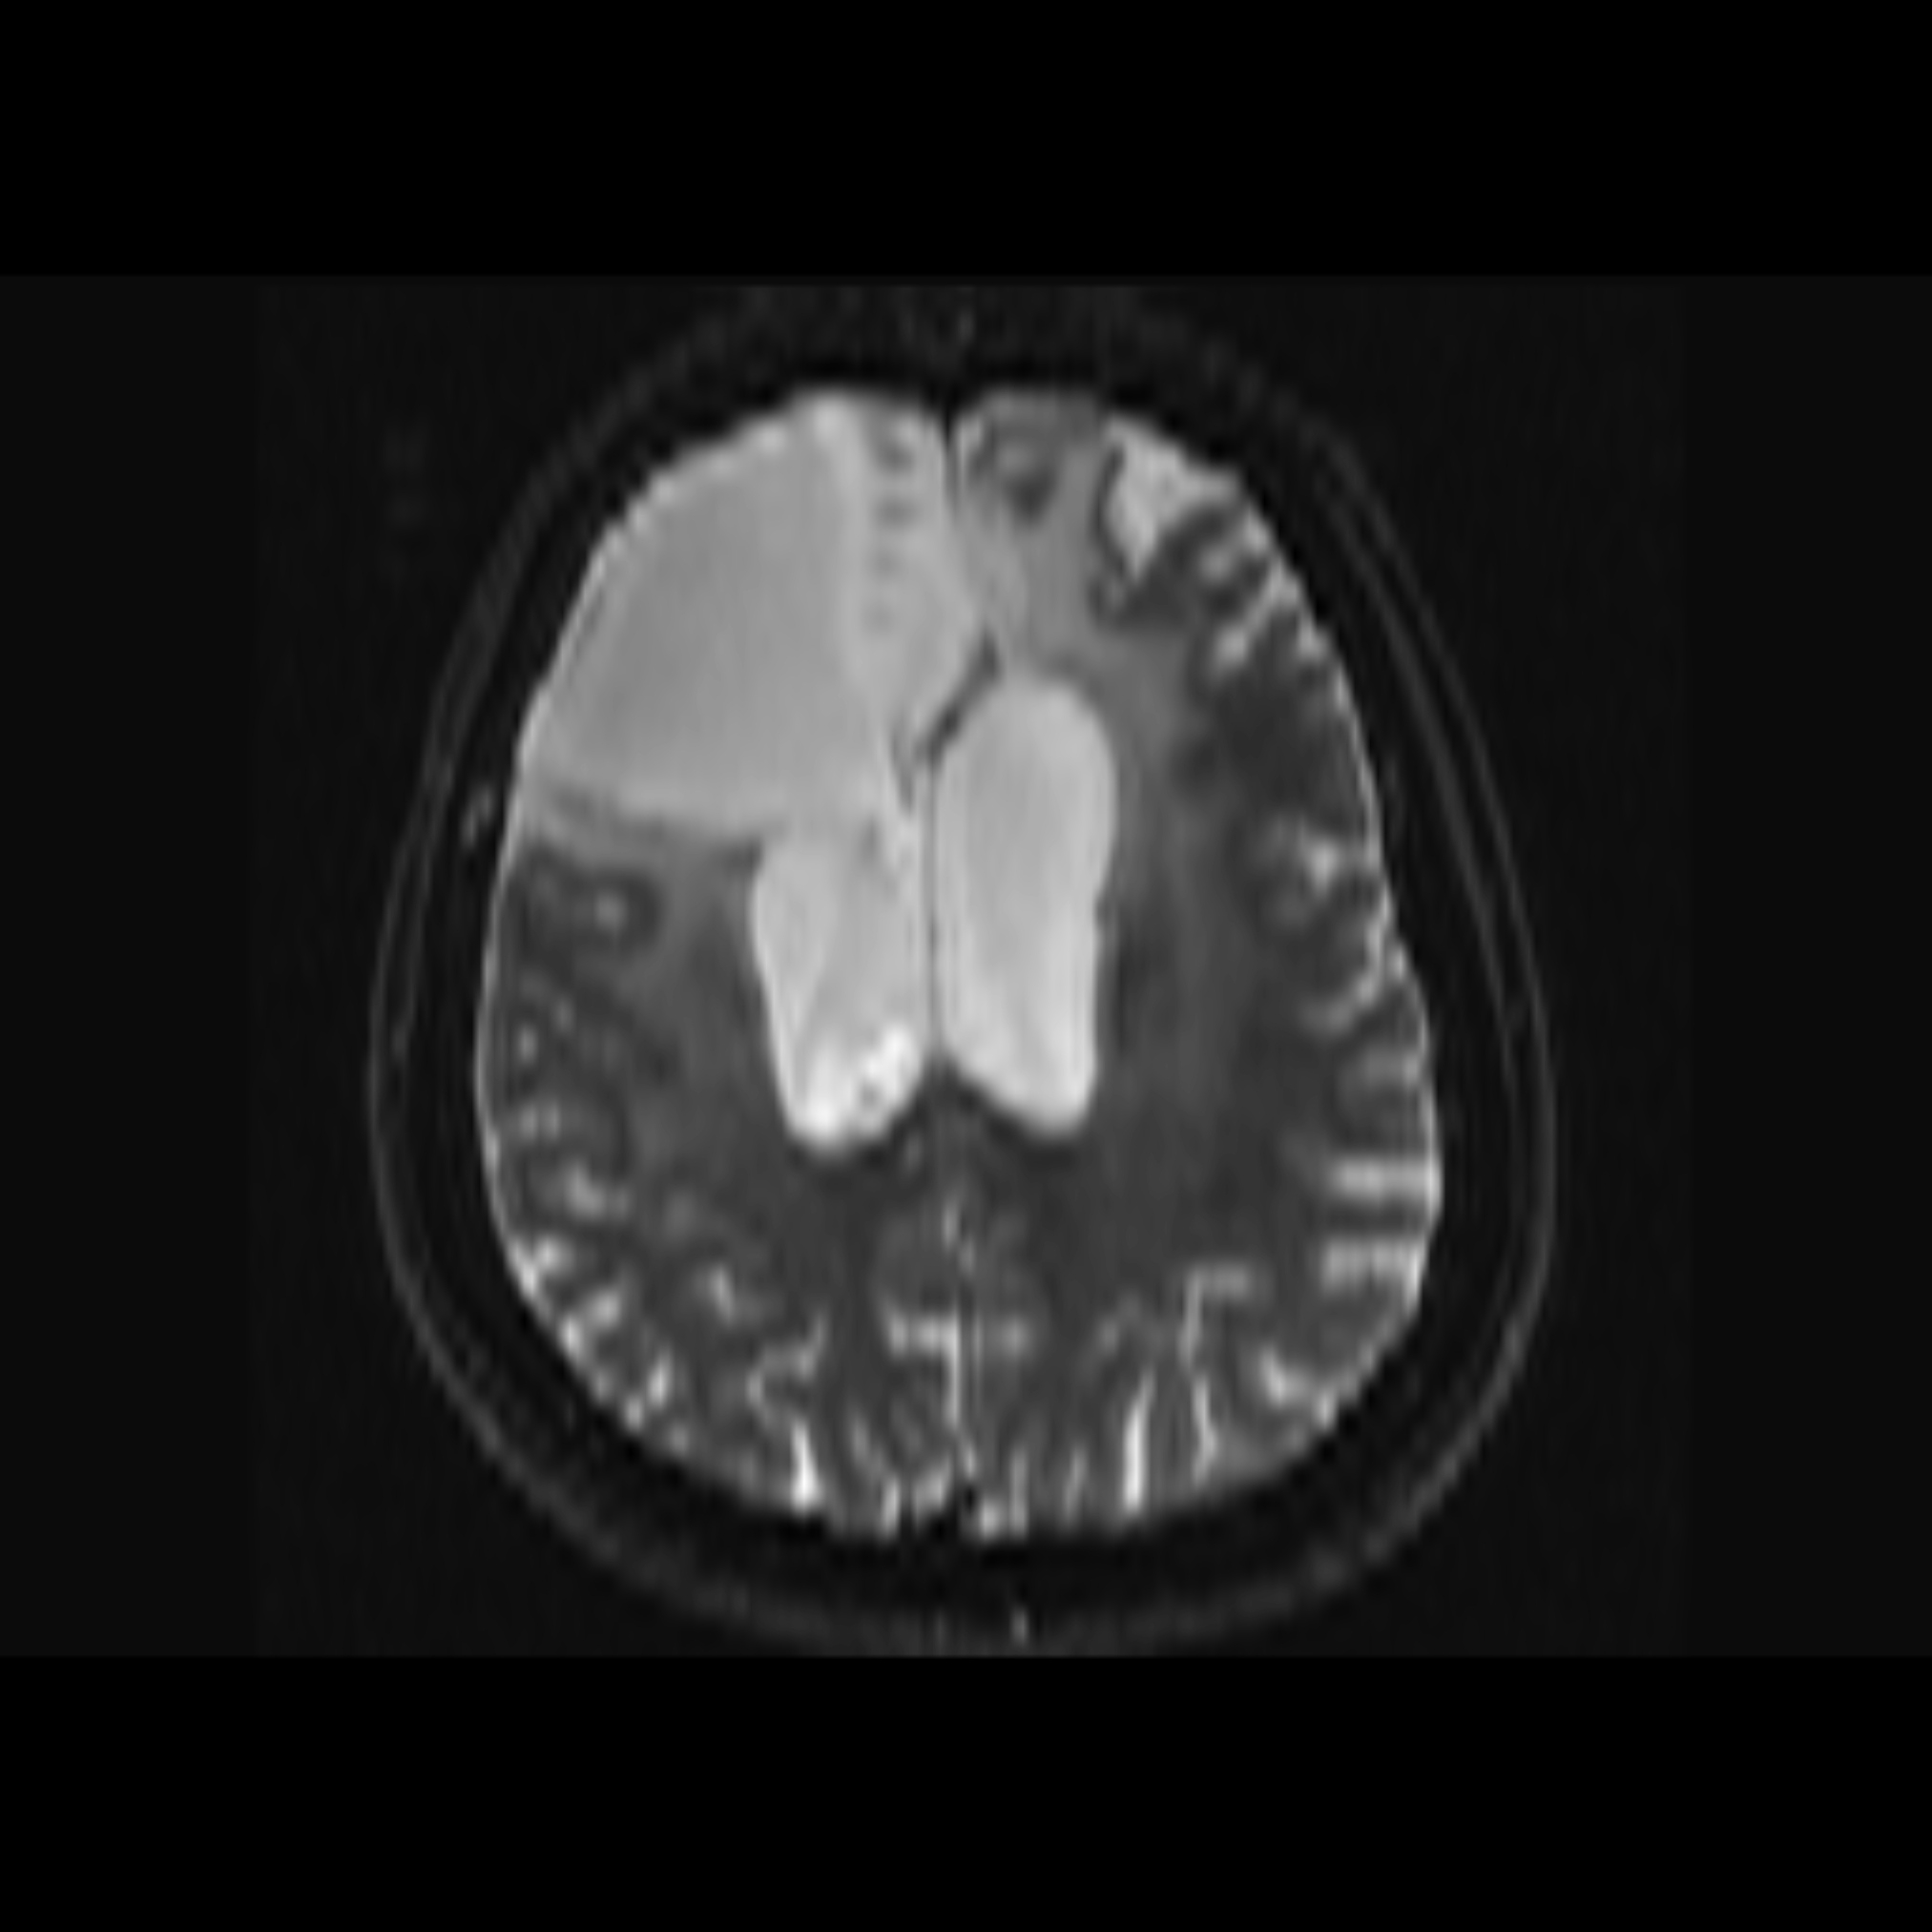
\includegraphics[width=\textwidth]{Figures/T2}
    \caption{\gls{T2}}\label{fig:T2w}
\end{subfigure}
\begin{subfigure}[t]{\figexamplewidth}
    \centering
    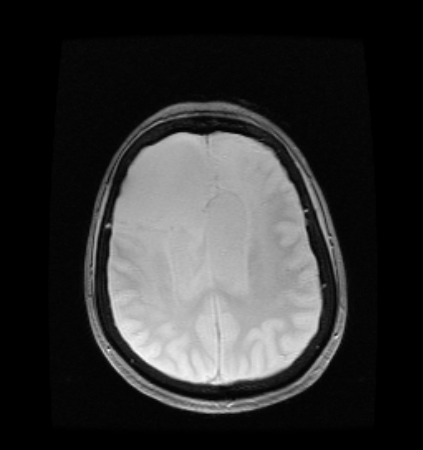
\includegraphics[width=\textwidth]{Figures/PD}
    \caption{\gls{PD}}\label{fig:PDw}
\end{subfigure}


\begin{subfigure}[t]{\figexamplewidth}
    \centering
    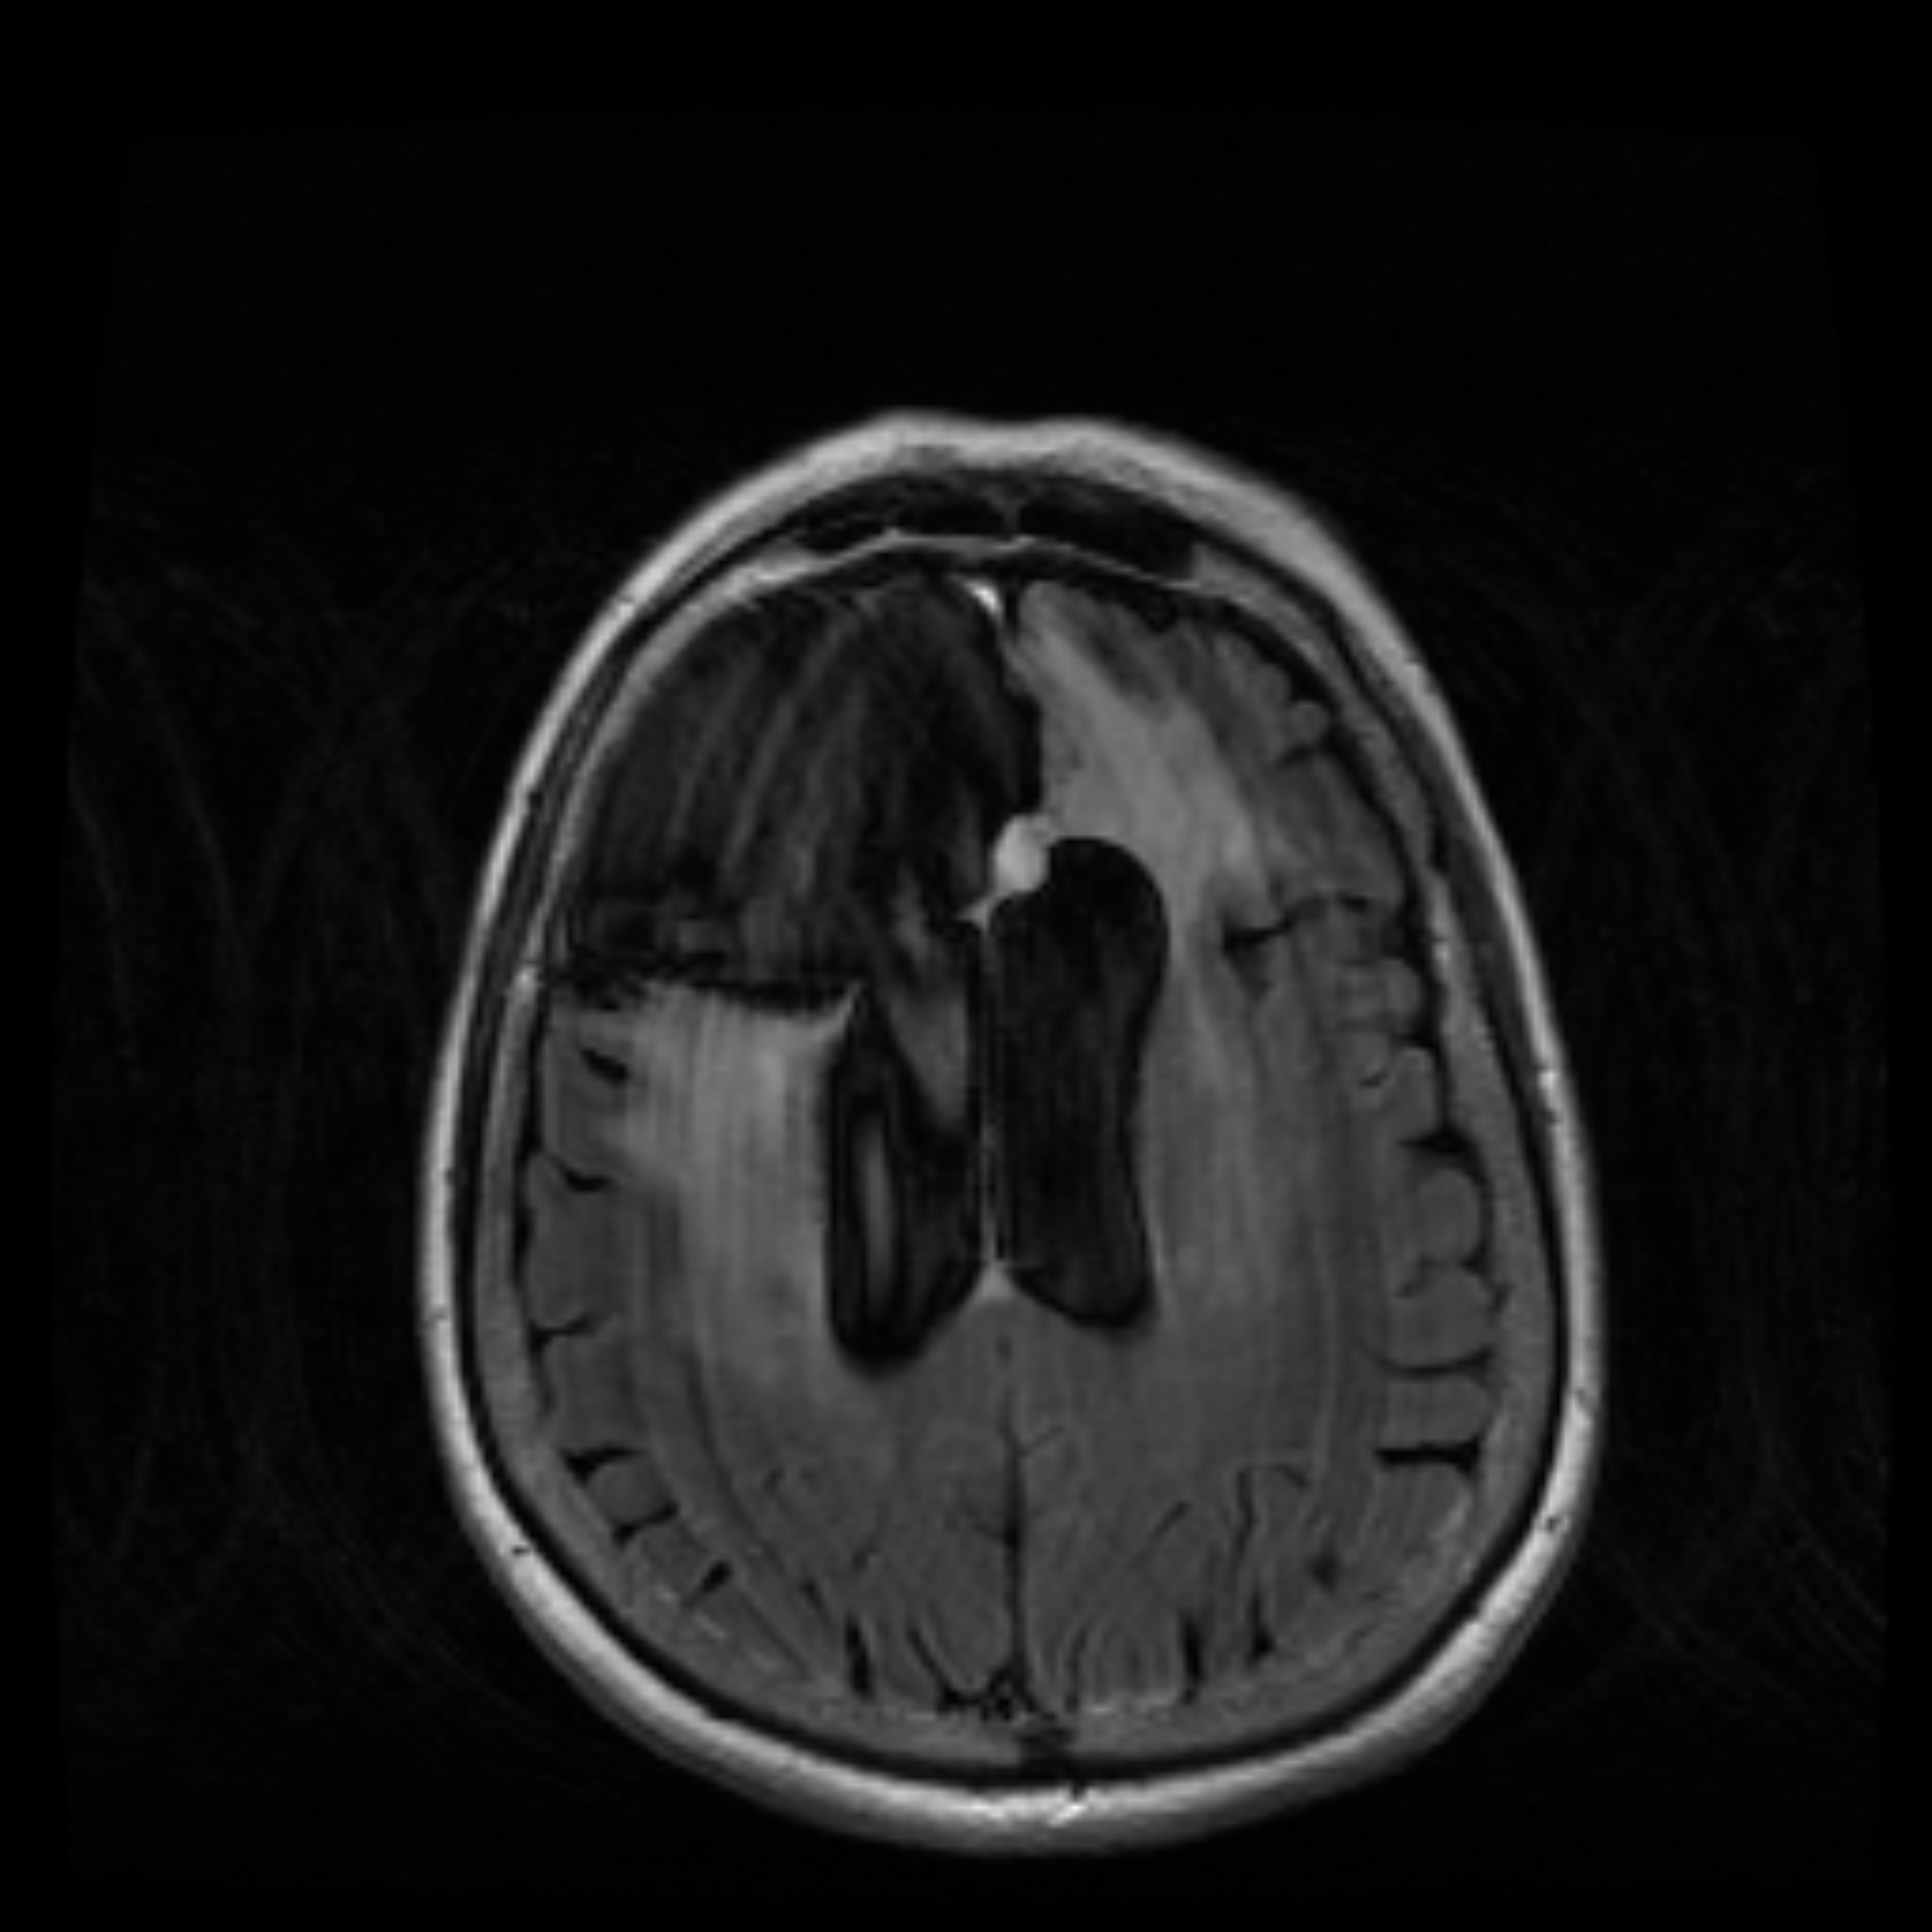
\includegraphics[width=\textwidth]{Figures/FLAIR}
    \caption{\gls{FLAIR}}\label{fig:FLAIR}
\end{subfigure}
\begin{subfigure}[t]{\figexamplewidth}
    \centering
    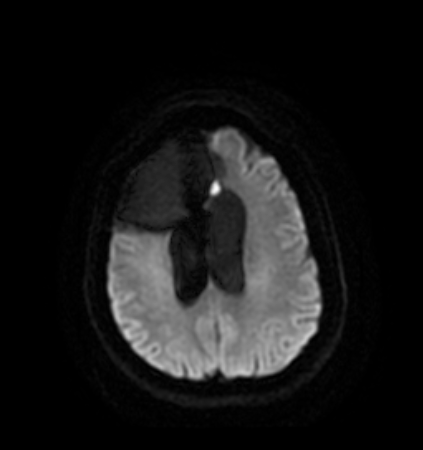
\includegraphics[width=\textwidth]{Figures/DWI}
    \caption{\gls{DWI}}\label{fig:DWI}
\end{subfigure}
\begin{subfigure}[t]{\figexamplewidth}
    \centering
    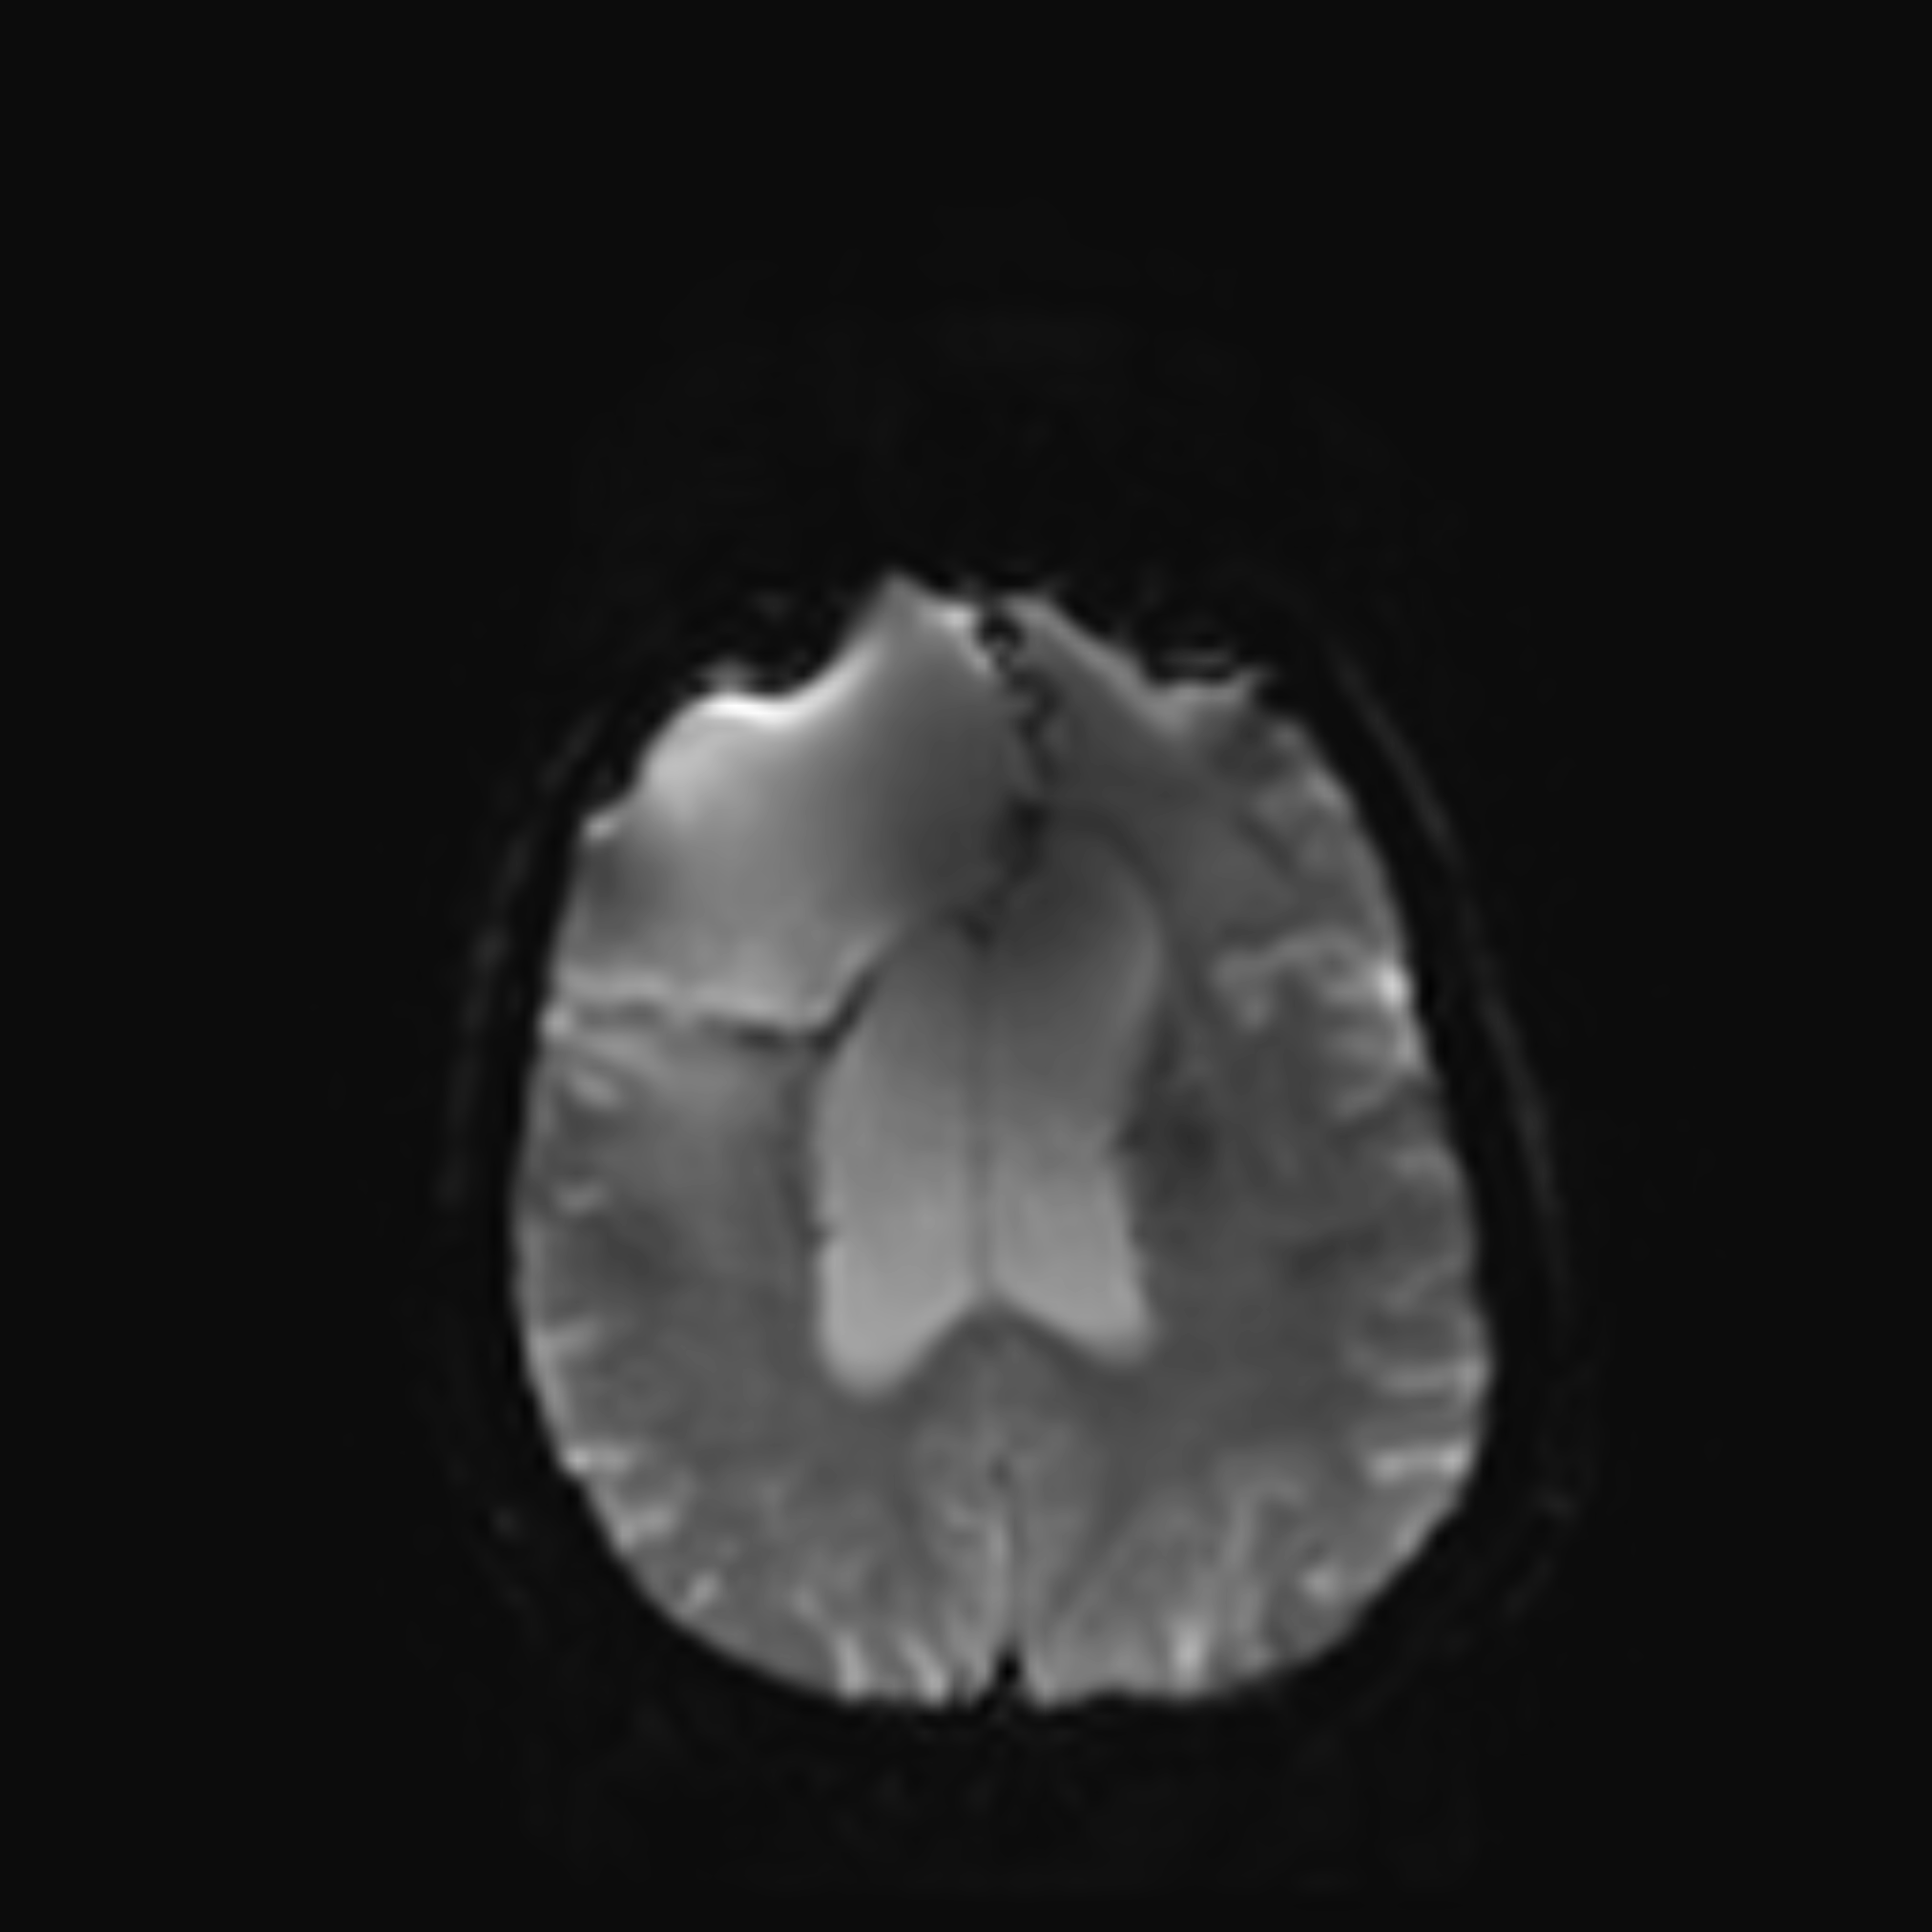
\includegraphics[width=\textwidth]{Figures/DSC}
    \caption{\gls{DSC}}\label{fig:PWI-DSC}
\end{subfigure}
\begin{subfigure}[t]{\figexamplewidth}
    \centering
    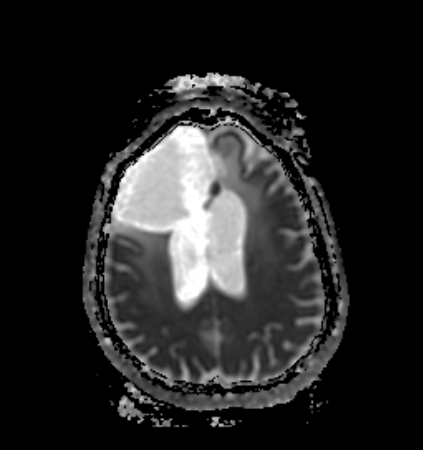
\includegraphics[width=\textwidth]{Figures/DERIVED}
    \caption{Derived (ADC)}\label{fig:Derived}
\end{subfigure}
\caption{Examples of the different \glspl{type} for a single \gls{sub} from the \gls{BTtest}}\label{fig:seq_examples}
\end{figure}


\subsubsection{\gls{NTTS}}

In order to evaluate the results of the algorithm on non-\gls{tumor} brain imaging, we used the \gls{ADNI} \gls{ds} (\url{adni.loni.usc.edu}).
The \gls{ADNI} was launched in 2003 as a public-private partnership, led by Principal Investigator Michael W. Weiner, MD.
The primary goal of \gls{ADNI} has been to test whether serial magnetic resonance imaging, positron emission tomography, other biological markers, and clinical and neuropsychological assessment can be combined to measure the progression of mild cognitive impairment and early Alzheimer's disease.
For up-to-date information, see \url{adni-info.org}.

We used the baseline and screening data of \num{1318} \glspl{sub}, resulting in \num{7227} \glspl{scan}.
These \glspl{scan} originated from \num{67} different \glspl{site} and were acquired on \num{23} different scanner models from \num{3} different vendors (GE, Philips, and Siemens).
Details of the \gls{NTTS} are presented in \cref{tab:data_adni}.
Since no contrast is administered to \glspl{sub} in the \gls{ADNI} study, there are no \gls{T1C} or \gls{DSC} \glspl{scan} in this \gls{ds}.
The \gls{ADNI} \gls{ds} does include \gls{ASL}, however since our algorithm was not designed to recognize these \glspl{scan}, they were excluded.
The derived maps from these \gls{ASL} \glspl{scan} were included since the derived category encompasses all diffusion and perfusion derived imaging.
These \gls{ASL} derived maps explain the \num{47} 3D \glspl{scan} in \cref{tab:data_adni}.

\begin{table}[htbp]
    \centering


    \setlength\scantablewidth{0.6cm}
    \setlength\datasetsep{20pt}
    \setlength\totaldata{0.8cm}

    \setlength{\tabcolsep}{3pt}

    \begin{tabular}{L{1.78cm}S[table-format=4.0]S[table-format=4.0]S[table-format=4.0]S[table-format=4.0]S[table-format=4.0]}
    \toprule
     &\multicolumn{5}{c}{\textbf{\Acrlong{NTTS}}}\\
    \cmidrule(l){2-6}
    \textbf{\Acrshort{type}} & {Ax} & {Cor} & {Sag} & {3D} & {Total}\\
     \midrule
     \acrshort{T1}       & 0    & 0    & 276  & 2380 & 2656\\
     \acrshort{T1C}      & 0    & 0    & 0    & 0    & 0   \\
     \acrshort{T2}       & 1725 & 488  & 5    & 0    & 2218\\
     \acrshort{PD}       & 1069 & 0    & 0    & 0    & 1069\\
     \acrshort{FLAIR}    & 1    & 0    & 3    & 488  & 492 \\
     \acrshort{DWI}      & 558  & 0    & 2    & 0    & 560   \\
     \acrshort{DSC}      & 0    & 0    & 0    & 0    & 0   \\
     Derived        & 183  & 0    & 2    & 47   & 232 \\
     \midrule
     \textbf{Total} & 3536 & 488  & 288  & 2915 & 7227\\
     \bottomrule
    \end{tabular}
    \caption{Overview of data in the \acrlong{NTTS}. The number of \glspl{scan} for each \gls{type} and the different spatial orientations (axial, coronal, sagittal, and 3D) are specified}\label{tab:data_adni}
\end{table}

\subsection{\acrlong{DDS}}
The pipeline of our proposed method, \gls{DDS}, consisted of three phases:
\begin{enumerate}
    \item Pre-processing: prepare the \glspl{scan} as an input for the \gls{CNN}
    \item \Gls{type} prediction: obtain the predicted \gls{type} using the \gls{CNN}
    \item Post-processing: use the predictions to sort the \gls{ds}
\end{enumerate}

By passing a \gls{ds} through this pipeline, it can be turned into a \gls{BIDS} compliant \gls{ds}, or it can be structured according to a user-defined layout.
If one chooses to create a \gls{BIDS} compliant \gls{ds}, the \glspl{scan} are stored as \gls{NIFTI} files; if a user-defined structure is used, the \glspl{scan} are stored as \gls{DICOM} files.
An overview of the \gls{DDS} pipeline is presented in \cref{fig:DDS_pipeline}.

\begin{figure}
\centering

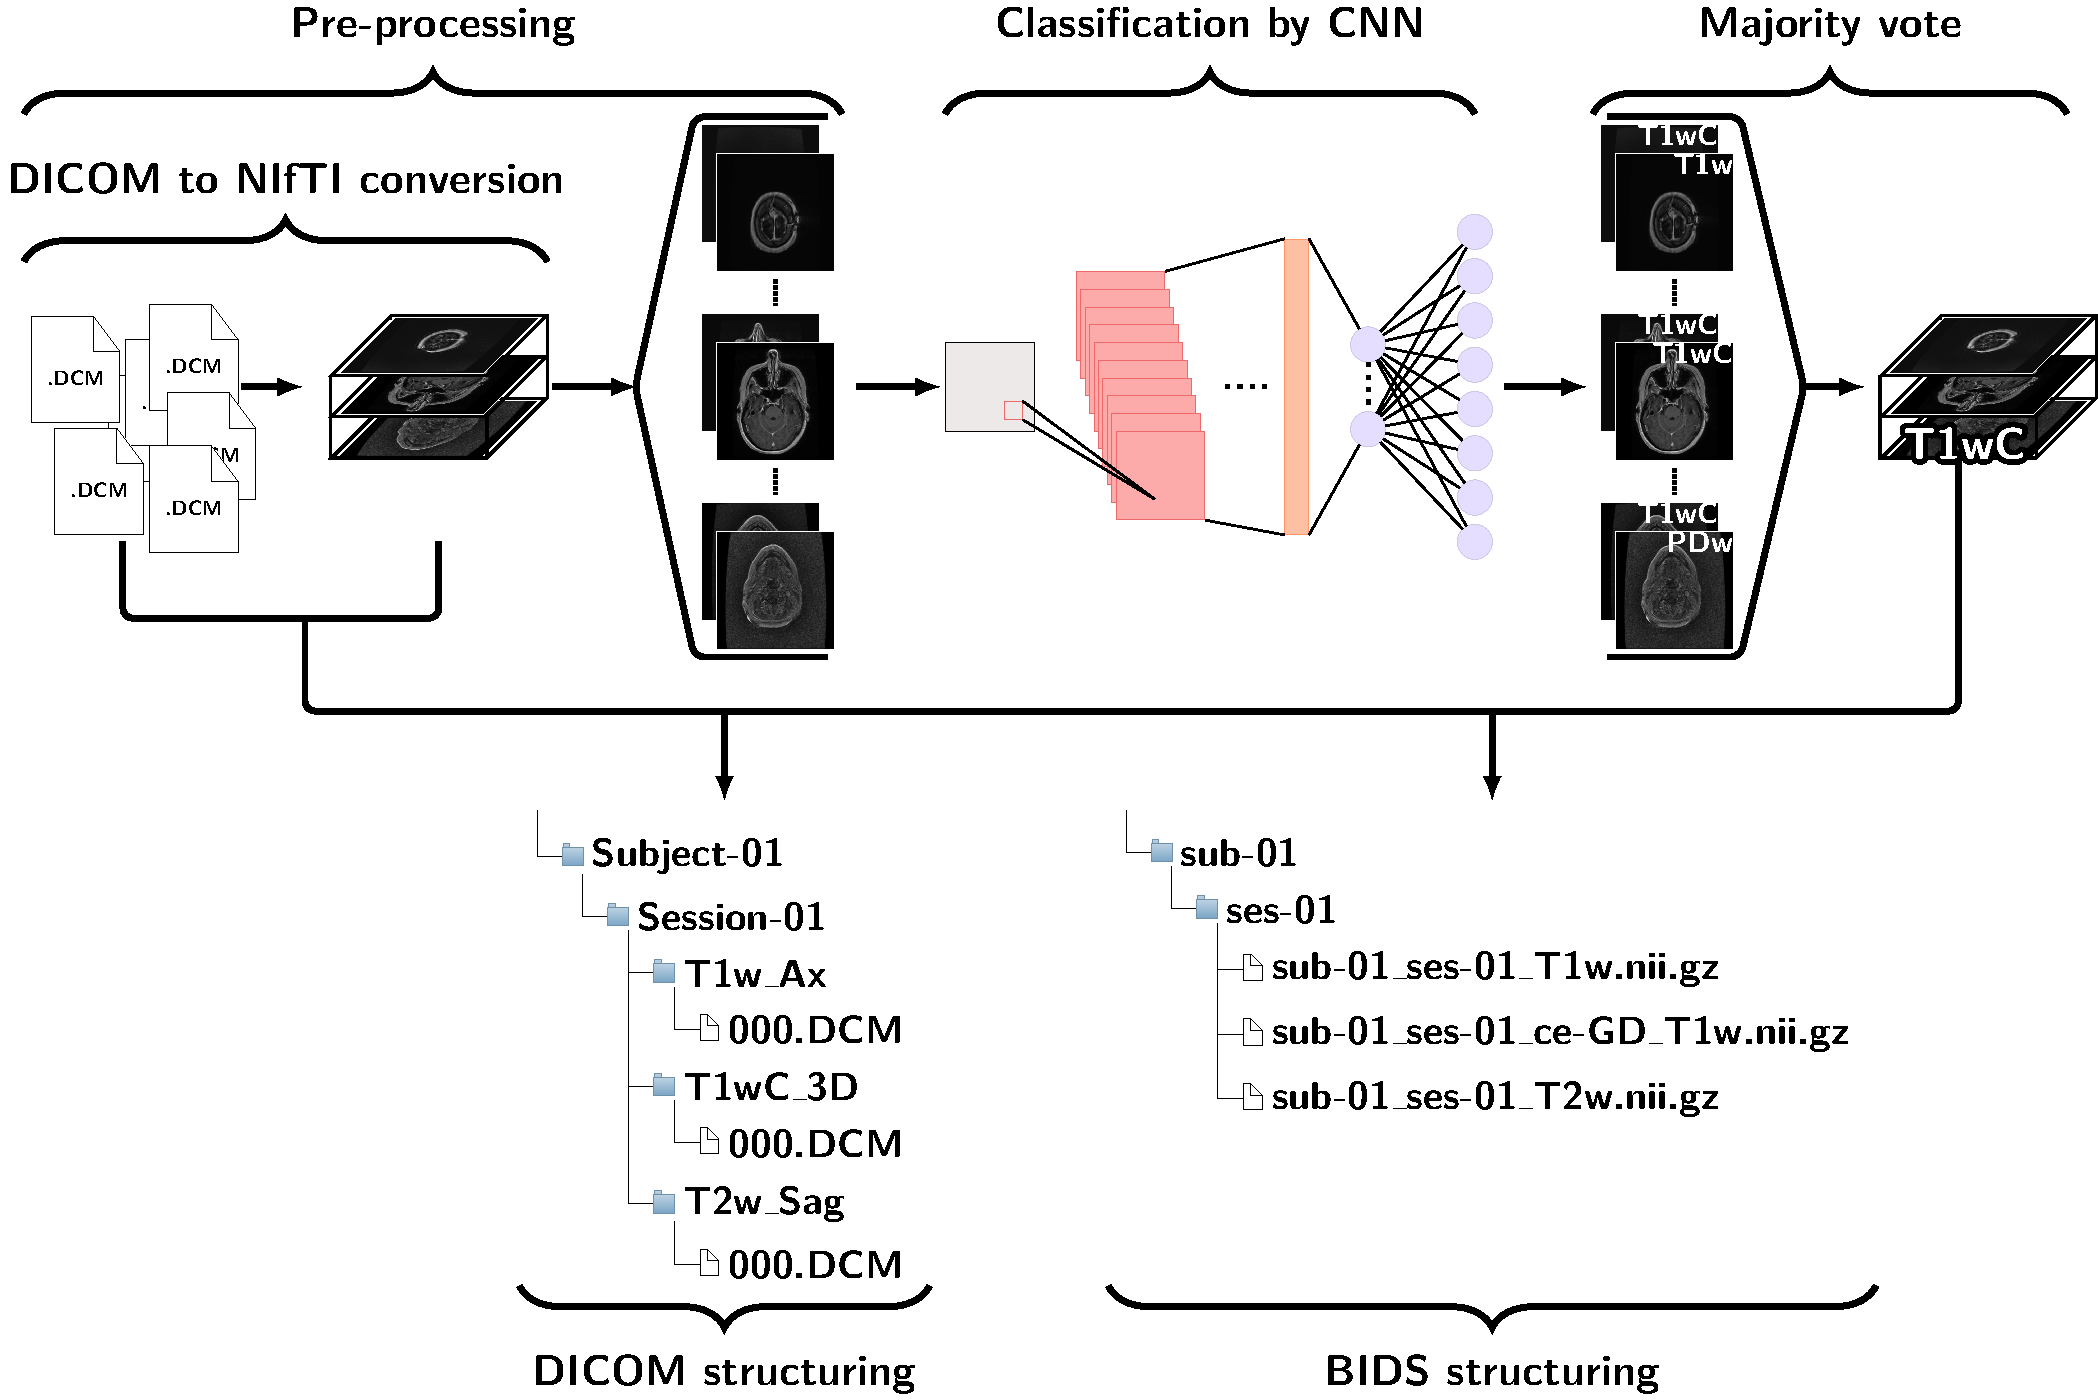
\includegraphics[width=\textwidth]{Figures/DDS_pipeline.pdf}
\caption{Overview of the \gls{DDS} pipeline.
\Glspl{scan} are first converted from \gls{DICOM} to \gls{NIFTI} format and pre-processed.
During the pre-processing the \gls{scan} is split into \num{25} individual \glspl{slice}, that are then classified as one of eight \glspl{type} by the \gls{CNN}.
The predictions of the individual \glspl{slice} are combined in a majority vote and the predicted \gls{type} of each \gls{scan} is used to structure the \gls{ds}.
\gls{DDS} can structure either the original \gls{DICOM} files, or the \gls{NIFTI} files.
In the last case the \gls{ds} turns into \gls{BIDS} compliant \gls{ds}}
\label{fig:DDS_pipeline}

\end{figure}

\subsubsection{Pre-processing}
\label{sec:preprocessing}
As a first pre-processing step, all \gls{DICOM} files were converted to \gls{NIFTI} format using dcm2niix \autocite{li2016first}, as this simplifies the further processing of the \glspl{scan}.
This step was skipped for the \gls{USIGT} and \gls{BITE} \glspl{ds}, as these were already provided in \gls{NIFTI} format (no \gls{DICOM} files were available).

In the next step, the number of dimensions of each \gls{scan} was automatically determined.
Although most \glspl{scan} were 3-dimensional, some \glspl{scan} happened to be 4-dimensional.
This was the case for some \gls{DWI} \glspl{scan}, which consisted of multiple b-values and potentially b-vectors, and for some \gls{DSC} \glspl{scan}, which contained multiple time points.
If a \gls{scan} was 4-dimensional, the first (3D) element of the sequence was extracted and was subsequently used instead of the full 4-dimensional \gls{scan}.
This extraction was done to make sure that the \gls{CNN} would also recognize \glspl{type} that generally contain repeats in situations where this was not the case.
For example, this could be the case when the different b-values of a \gls{DWI} \gls{scan} were stored as multiple, separate (3D) \glspl{scan} instead of a single (4D) \gls{scan}.
Since the information that a \gls{scan} is 4-dimensional can aid the algorithm in recognizing the \gls{type}, a \say{4D} label was attached to each \gls{scan}.
This 4D label was set to 1 if the \gls{scan} was 4-dimensional, and to 0 if it was not.

All \glspl{scan} were then reoriented to match the orientation of a common template using FSL's reorient2std \autocite{jenkinson2012fsl}.
After this step, the \glspl{scan} were resampled to $ 256 \times 256 \times 25$ voxels, using cubic b-spline interpolation, while maintaining the original field of view.
All of these resampled (3D) \glspl{scan} were split into (2D) \glspl{slice}, resulting in \num{25} individual \glspl{slice} of $256 \times 256$ voxels.
The \gls{slice} extraction was then followed by an intensity scaling of each \gls{slice}.
The intensity was scaled such that the minimum intensity was 0, and the maximum intensity was \num{1} to compensate for intensity differences between \glspl{slice}.
These pre-processed \glspl{slice} were than used as input \glspl{sample} for the \gls{CNN}.
No data augmentation was used, as the large number of \glspl{scan} and different data sources that were used to train the algorithm already ensured sufficient natural variation in the \glspl{sample}, obviating the need for additional augmentation.

After applying these pre-processing steps, the \gls{BTtrain} consisted of \num{276625} \glspl{sample}, the \gls{BTtest} consisted of \num{59225} \glspl{sample}, and the \gls{NTTS} consisted of \num{180675} \glspl{sample}.

\subsubsection{Network}
\label{sec:network}

A \gls{CNN} was used to classify the \glspl{sample} into one of eight different \glspl{class}: \gls{T1}, \gls{T1C}, \gls{T2}, \gls{PD}, \gls{FLAIR}, \gls{DWI}, \gls{DSC}, or derived.
The architecture of the \gls{CNN} is shown in \cref{fig:sequence_architecture}.
This architecture was inspired by the VGG network \autocite{simonyan2014very}.

The network was implemented using TensorFlow 1.12.3 \autocite{abadi2016tensorflow}.
The cross-entropy between the predicted and ground truth labels was used as a loss function.
Weights were initialized using Glorot Uniform initialization \autocite{glorot2010understanding}.
We used Adam as an optimizer \autocite{kingma2014adam}, which started with a learning rate of \num{0.001} $\beta_1 = 0.9$, and $\beta_2=0.999$, as these were proposed as reasonable default values \autocite{kingma2014adam}.
The learning rate was automatically adjusted based on the training loss; if the training loss did not decrease during \num{3} epochs, the learning rate was decreased by a factor \num{10}, with a minimum learning rate of \num{1e-7}.
The network could train for a maximum of \num{100} epochs, and the network automatically stopped training when the loss did not decrease during \num{6} epochs.
We used a batch size of \num{32}.
We arrived at this \gls{CNN} design and these settings by testing multiple different options and selecting the best performing one.
Details about the optimization of the settings are presented in \cref{sec:experiments}, \cref{fig:brain_tumor_experiment}, and \cref{app:crossval}.

During the training of the network, all \glspl{slice} were inputted to the \gls{CNN} as individual \glspl{sample}, and no information about the (possible) relation between different \glspl{slice} was provided.
After training the network, the \gls{type} of a \gls{scan} was predicted by passing all \num{25} \glspl{slice} of the \gls{scan} through the \gls{CNN} and then combining these individual \gls{slice} predictions using a majority vote.

\begin{figure}
\centering

\resizebox{\textwidth}{!}{
\subimport{Figures/}{CNN_architecture.pgf}
}

\caption{The architecture of the \gls{CNN}. The convolutional blocks consisted of N 2D convolutional filters followed by batch normalization and a parametric rectified linear unit.
The output size of the convolutional blocks and pooling layers is specified}
\label{fig:sequence_architecture}
\end{figure}

\subsubsection{Post-processing}

Once the \gls{type} of each \gls{scan} is predicted, these predictions can then be used in (optional) post-processing steps to automatically structure the \gls{ds}.
We provide two options for the structured format:

\begin{itemize}
    \item Sort the original \gls{DICOM} files; this can be done in a user-defined folder structure.
    \item Sort the \gls{NIFTI} files; in this case the \gls{BIDS} format is used.
\end{itemize}

During the post-processing, the spatial orientation of the \gls{scan} (axial, coronal, sagittal, or 3D) is also determined based on the direction cosines (\gls{DICOM} tag (0020, 0037)), which can be used to define the structured layout when choosing to sort the \gls{DICOM} files.

\subsection{\acrlong{HC}}
\gls{HC}\footnote{\url{https://github.com/nipy/heudiconv}} is a heuristic-centric \gls{DICOM} converter, which uses information from the \gls{DICOM} tags, along with a user-defined heuristic file to organize an unstructured \gls{DICOM} \gls{ds} into a structured layout.
\gls{HC} is currently one of the most widespread, publicly available methods that can structure an unsorted \gls{DICOM} \gls{ds}.
Therefore, we used \gls{HC} as a benchmark so we could compare our method, which is based on the visual appearance of a \gls{scan}, with a method that is based on the metadata of a \gls{scan}.

Before \gls{HC} can be used to sort a \gls{ds}, one first needs to define the heuristic file, which is essentially a translation table between the metadata of a \gls{scan} and its \gls{type}.
This heuristic file is based on \gls{scan} metadata that is extracted from the \gls{DICOM} tags.
Available metadata includes image type, study description, series description, repetition time, echo time, size of the \gls{scan} along 4 dimensions, protocol name, and sequence name.
\gls{HC} also determines whether a \gls{scan} is motion-corrected or is a derived image, based on specific keywords being present in the image type \gls{DICOM} tag.
These characteristics can also be used in the heuristic file.
Although more \gls{scan} metadata can be used to define the heuristic, such as \gls{sub} sex and referring physician, we considered this metadata irrelevant for our purpose of \gls{type} prediction.
In addition, this kind of metadata was often missing due to anonymization.



\subsection{Experiments}
\label{sec:experiments}

\subsubsection{Evaluation of \gls{DDS}}

We performed two experiments in which we constructed and evaluated our method, to show the generalizability among different \glspl{ds}:

\begin{itemize}
    \item Experiment I: Algorithm trained on \gls{BTtrain} and tested on \gls{BTtest}
    \item Experiment II: Algorithm trained on \gls{BTset} (\gls{BTtrain} and \gls{BTtest}), and tested on \gls{NTTS}
\end{itemize}

In Experiment I we developed the algorithm and tried different \gls{CNN} architectures, pre-processing settings, and optimizer settings, collectively referred to as the model parameters, using a train/validation split of the \gls{BTtrain}.
We then selected the best performing model parameters and trained a \gls{CNN} using the whole \gls{BTtrain}.
Once the model was trained, its performance was evaluated on the \gls{BTtest}.
In Experiment I, the \gls{BTtest} was only used to evaluate the results and was left untouched during the development and training of the algorithm.
\cref{fig:brain_tumor_experiment} shows an overview of the model parameter selection, training and testing steps, and the data used in Experiment I.
More details about the selection of the optimal model parameters and the results of other model parameters can be found in \cref{app:crossval}.

In Experiment II we used the \gls{NTTS} as a test set to see if our method also generalizes to \glspl{scan} in which no brain \gls{tumor} was present.
In this experiment, we trained the \gls{CNN} using the whole \gls{BTset} (a combination of all the data in the \gls{BTtrain} and \gls{BTtest}) and then evaluated the performance of the model on the \gls{NTTS}.
No model parameter selection was done in this experiment, instead the optimal model parameters that were obtained from Experiment I were used.
Thus, apart from training the \gls{CNN} on a larger \gls{ds}, the methods used in Experiment I and Experiment II were the same.
\cref{fig:adni_experiment} shows an overview of the training and testing steps and the data used in Experiment II.
In this experiment, no \gls{T1C} and \gls{DSC} \glspl{scan} were present in the test set, however in a real-world setting one may not know a priori whether these \glspl{type} were present or absent.
Thus, we still allowed the model to predict the \gls{type} as one of these \glspl{class} to mirror this realistic setting.

\begin{sidewaysfigure}[htbp]
\centering
\resizebox{0.9\textwidth}{!}{
    \subimport{Figures/}{brain_tumor_experiment.pgf}
}
\caption{Overview of Experiment I. In this experiment, the \gls{BTtrain} was used to obtain the optimal model parameters and to train the algorithm. The trained model was then evaluated on the \gls{BTtest}}
\label{fig:brain_tumor_experiment}
\end{sidewaysfigure}

\begin{sidewaysfigure}[htbp]
\centering

\resizebox{0.9\textwidth}{!}{
\subimport{Figures/}{adni_experiment.pgf}
}

\caption{Overview of Experiment II. In this experiment the \gls{BTset} was used to train the algorithm, and the trained model was then evaluated on the \gls{NTTS}}
\label{fig:adni_experiment}
\end{sidewaysfigure}

To evaluate the performance of our algorithm, we calculated the overall accuracy and the per-class accuracy of the classification.
The overall accuracy was defined as the number of correctly predicted \glspl{scan} divided by the total number of \glspl{scan}.
The per-class accuracy was defined as the number of correctly predicted \glspl{scan} of a specific \gls{type} divided by the total number of \glspl{scan} of that \gls{type}.
We also computed the confusion matrices, which show the relationship between the ground truth and predicted \gls{class}.

To visualize which parts of the \gls{slice} contributed most to the prediction of the \gls{CNN}, we generated saliency maps \autocite{simonyan2014deep}.
Saliency maps were generated by calculating the gradient of a specific \gls{class} with respect to each input pixel, thus giving a measure of the contribution of each pixel.
To obtain sharper maps, we used guided backpropagation \autocite{springenberg2015striving} and applied a rectified linear activation to the obtained maps.
Saliency maps were generated for all \glspl{slice} of the \glspl{scan} of the example \gls{sub} shown in \cref{fig:seq_examples}, based on the trained model from Experiment I.
Additional saliency maps were generated for 20 \glspl{sample} of each \gls{type} that were randomly selected from the test sets of Experiment I and Experiment II.
The saliency maps for the \glspl{sample} from Experiment I were generated using the \gls{CNN} trained in Experiment I, and for the \glspl{sample} from Experiment II the \gls{CNN} trained in Experiment II was used.
By generating saliency maps for multiple \glspl{sample}, we could show the behavior of our algorithm for different \gls{scan} appearances.
Some of these \glspl{sample} contained \glspl{tumor}, contained imaging artifacts or had a low image quality.
Thus, these saliency maps also showed the robustness of our algorithm to unusual \gls{scan} appearance.
To gain some insight into the behavior of each convolutional layer we determined the feature maps of each convolutional layer.
We calculated the feature maps for the \gls{T1} \gls{slice} shown in \cref{fig:seq_examples} by passing it through the network and determining the output of each filter after each convolutional layer.


\subsubsection{Comparison with \acrlong{HC}}

We compared the performance of \gls{HC} and \gls{DDS} using the data from Experiment I, since the data in Experiment II did not include all \glspl{type}.
When using \gls{HC}, only the \glspl{scan} which were available in \gls{DICOM} format could be processed.
This meant that the \glspl{scan} from the \gls{USIGT} \gls{ds} were removed from the \gls{BTtrain}, and the \glspl{scan} from the \gls{BITE} \gls{ds} were removed from the \gls{BTtest}, as these were not available in \gls{DICOM} format.
Thus,  86 \glspl{scan} (43 \gls{T1C} and 43 \gls{FLAIR}) were removed from the \gls{BTtrain} and 27 \glspl{scan} (all \gls{T1C}) were removed from the \gls{BTtest}, reducing the train set to 10979 \glspl{scan} and the test set to 2342 \glspl{scan}.

To construct our heuristic, we first extracted all the relevant \gls{DICOM} tags from the \glspl{scan} in the \gls{BTtrain}, see \cref{tab:heuditags}.
\cref{tab:heuditags} also shows the number of unique occurrences for text-based tags and the distribution of the numerical tags in the \gls{BTtrain}.
An iterative approach was followed to construct the heuristic, where rules were added or adjusted until the performance of \gls{HC} on the \gls{BTtrain} could no longer be increased, see \cref{fig:heudiconv_experiment}.
Our initial heuristic was a simple one, based solely on certain text being present in the series description.
For example, if the text \say{T1} was present in the series description, it was considered a \gls{T1} \gls{scan}.

To compare the performance of \gls{HC} with the performance of \gls{DDS} the overall accuracy and per-class accuracy of the \gls{type} predictions obtained from \gls{HC} were calculated.


\begin{table}[htbp]
 \centering
  \begin{tabular}{L{5cm} l l l}
      \toprule
      \textbf{Tag description} & \textbf{Tag number}\\
      \midrule
      Image type & 0008,0008 & 72 unique instances\\
      Study description	 & 0008,1030 & 435 unique instances\\
      Series description & 0008,103E & 1215 unique instances\\
      Repetition time & 0018,0080 & Mean $\pm$ std: 3912 $\pm$ 4078\\
      Echo time & 0018,0081 & Mean $\pm$ std: 52.11 $\pm$ 48.9 \\
      Number of rows in image & 0028,0010 & Range: 128 - 1152\\
      Number of columns in image & 0028,0011 & Range: 128 - 1152\\
      \bottomrule
  \end{tabular}
  \caption{DICOM tag numbers and descriptions of the DICOM tags extracted for the \acrlong{HC} heuristic. For text-based tags the number of unique instances is shown and for numerical-based tags the distribution is shown, based on the \glspl{scan} in the \gls{BTtrain}}\label{tab:heuditags}
\end{table}


\begin{sidewaysfigure}
\centering

\resizebox{0.9\textwidth}{!}{
\subimport{Figures/}{heudiconv_experiment.pgf}
}

\caption{Overview of the \gls{HC} experiment. In this experiment the \glspl{scan} from the \gls{BTtrain} that were available in \gls{DICOM} format were used to construct the heuristic file. \gls{HC} used this heuristic file to predict the \gls{type} of the \glspl{scan} from the \gls{BTtest} which were available in \gls{DICOM} format}
\label{fig:heudiconv_experiment}
\end{sidewaysfigure}


\section{Results}

\subsection{Experiment I - Evaluation on \gls{BTset}}
The results from Experiment I (evaluation on the \gls{BTtest}, containing \glspl{scan} of \glspl{sub} with brain \glspl{tumor}) are reported in \cref{tab:seqacc}.
The network was trained for 96 epochs.
In this experiment our method achieved an overall accuracy of \per{98.7}.

The highest per-class accuracy was achieved for the \gls{PD} and \gls{DSC} \glspl{scan} (\per{100.0} for both), whereas the \gls{FLAIR} \glspl{scan} had the lowest accuracy (\per{93.0}).
The confusion matrices show that most of the incorrectly predicted \gls{FLAIR} \glspl{scan} were classified as \gls{T1} \glspl{scan} (see  \cref{app:confusionmatrices}).
\cref{app:sliceresults} shows the performance of our method on a per-\gls{slice} basis before the majority vote has taken place to determine the \gls{scan} \gls{class}, which shows that the per-\gls{slice} accuracy is lower than the per-\gls{scan} accuracy.
This is not surprising since there are \glspl{slice} in a \gls{scan} from which it is almost impossible to determine the \gls{type} even for a human (for example, the most superior and inferior \glspl{slice}).


\subsection{Experiment II - Evaluation on \gls{NTTS}}
The results from Experiment II (evaluation on the \gls{NTTS}, containing \glspl{scan} of \glspl{sub} without brain \glspl{tumor}) are reported in \cref{tab:seqacc}.
Just like in Experiment I the network was trained for 96 epochs.
In this experiment our method achieved an overall accuracy of \per{98.5}.
It took approximately \num{22} hours to train the network of this experiment using an Nvidia Titan V GPU with 12 GB memory.

The highest per-class accuracy was achieved for the \gls{T1} \glspl{scan} (\per{100.0}), whereas the \gls{T2} \glspl{scan} had the lowest accuracy (\per{95.1}).
Most of the incorrectly predicted \gls{T2} \glspl{scan} were predicted as \gls{T1C} or \gls{PD} \glspl{scan}.
Furthermore, although no \gls{T1C} and \gls{DSC} \glspl{scan} were present in the test set used in this experiment, our method incorrectly classified 40 \glspl{scan} as \gls{T1C} (mainly \gls{T2} \glspl{scan}) and 3 \glspl{scan} as \gls{DSC} \glspl{scan} (all \gls{DWI} \glspl{scan}).
The full confusion matrix can be found in \cref{app:confusionmatrices}.

\subsection{Focus of the network}
\cref{fig:seq_gradcam} shows the saliency maps for the different \glspl{type}, for the same \glspl{slice} as in \cref{fig:seq_examples}.
For most \glspl{type}, the \gls{CNN} seemed to focus on the ventricles, the \gls{CSF} around the skull, the nose, and the eyes.
For the \gls{PD} \gls{slice}, the \gls{CNN} did not have a specific focus on the ventricles and did not seem to have a particular focus inside the brain.
The \gls{DWI} and derived \glspl{slice} also showed some focus outside of the skull, probably because of the artifacts outside of the skull that these \glspl{type} often feature (as can be seen in \cref{fig:DWI-DCam}).
We have created saliency maps for all 25 \glspl{slice} of the \glspl{scan} shown in \cref{fig:seq_examples}, which are shown in \cref{app:saliency}.
For most other \glspl{slice} the focus of the \gls{CNN} was the same as for the \glspl{slice} from \cref{fig:seq_gradcam}.
Furthermore, the presence of a \gls{tumor} did not disturb the prediction as also evidenced by the high accuracy achieved in Experiment I.
Only on the most superior and inferior \glspl{slice} did the \gls{CNN} struggle, probably due to the fact that the brain was barely visible on those \glspl{slice}.

Additional saliency maps for randomly selected \glspl{sample} from the test sets of Experiment I and Experiment II are shown in \cref{app:artifactsaliency}.
These examples show that our method is robust to heterogeneity in the visual appearance of the \glspl{scan}, as well as to the presence of \glspl{tumor}, the presence of imaging artifacts, and poor image quality.
This is demonstrated by the fact that the \gls{CNN} focused on the same brain structures for almost all of the \glspl{slice} and correctly predicted the \gls{type} even for \glspl{slice} with poor imaging quality or artifacts.
The feature maps of all convolutional layers are shown in \cref{app:filtervis}.
For the shallow convolutional layers, some filters seemed to detect the skull without looking at the brain tissue, whereas other layers seemed to focus more on specific brain structures such as the \gls{CSF}.
Interpreting the deeper convolutional layers gets harder as the feature maps of those layers have a lower resolution.

\begin{table}[htbp]
 \centering
  \begin{tabular}{lS[table-format=1.3]S[table-format=1.3]}
      \toprule
& {\textbf{Experiment I}} & {\textbf{Experiment II}}\\
    \midrule
  Overall    & 0.987 & 0.985\\
  \cmidrule{2-3}
  \acrshort{T1}        & 0.993 & 1.000\\
  \acrshort{T1C}       & 0.997 & {\NA}\\
  \acrshort{T2}        & 0.990 & 0.965\\
  \acrshort{PD}        & 1.000 & 0.998\\
  \acrshort{FLAIR}  & 0.930 & 0.951\\
  \acrshort{DWI}        & 0.991 & 0.995\\
  \acrshort{DSC}    & 1.000 & {\NA}\\
  Derived    & 0.994 & 0.983\\
  \bottomrule
  \end{tabular}
  \caption{Overall accuracy and per-class accuracy achieved by \gls{DDS} in Experiment I and Experiment II}\label{tab:seqacc}

\end{table}


\begin{figure}
    \centering

    \setlength{\figexamplewidth}{0.22\textwidth}

    \begin{subfigure}[t]{\figexamplewidth}
        \centering
        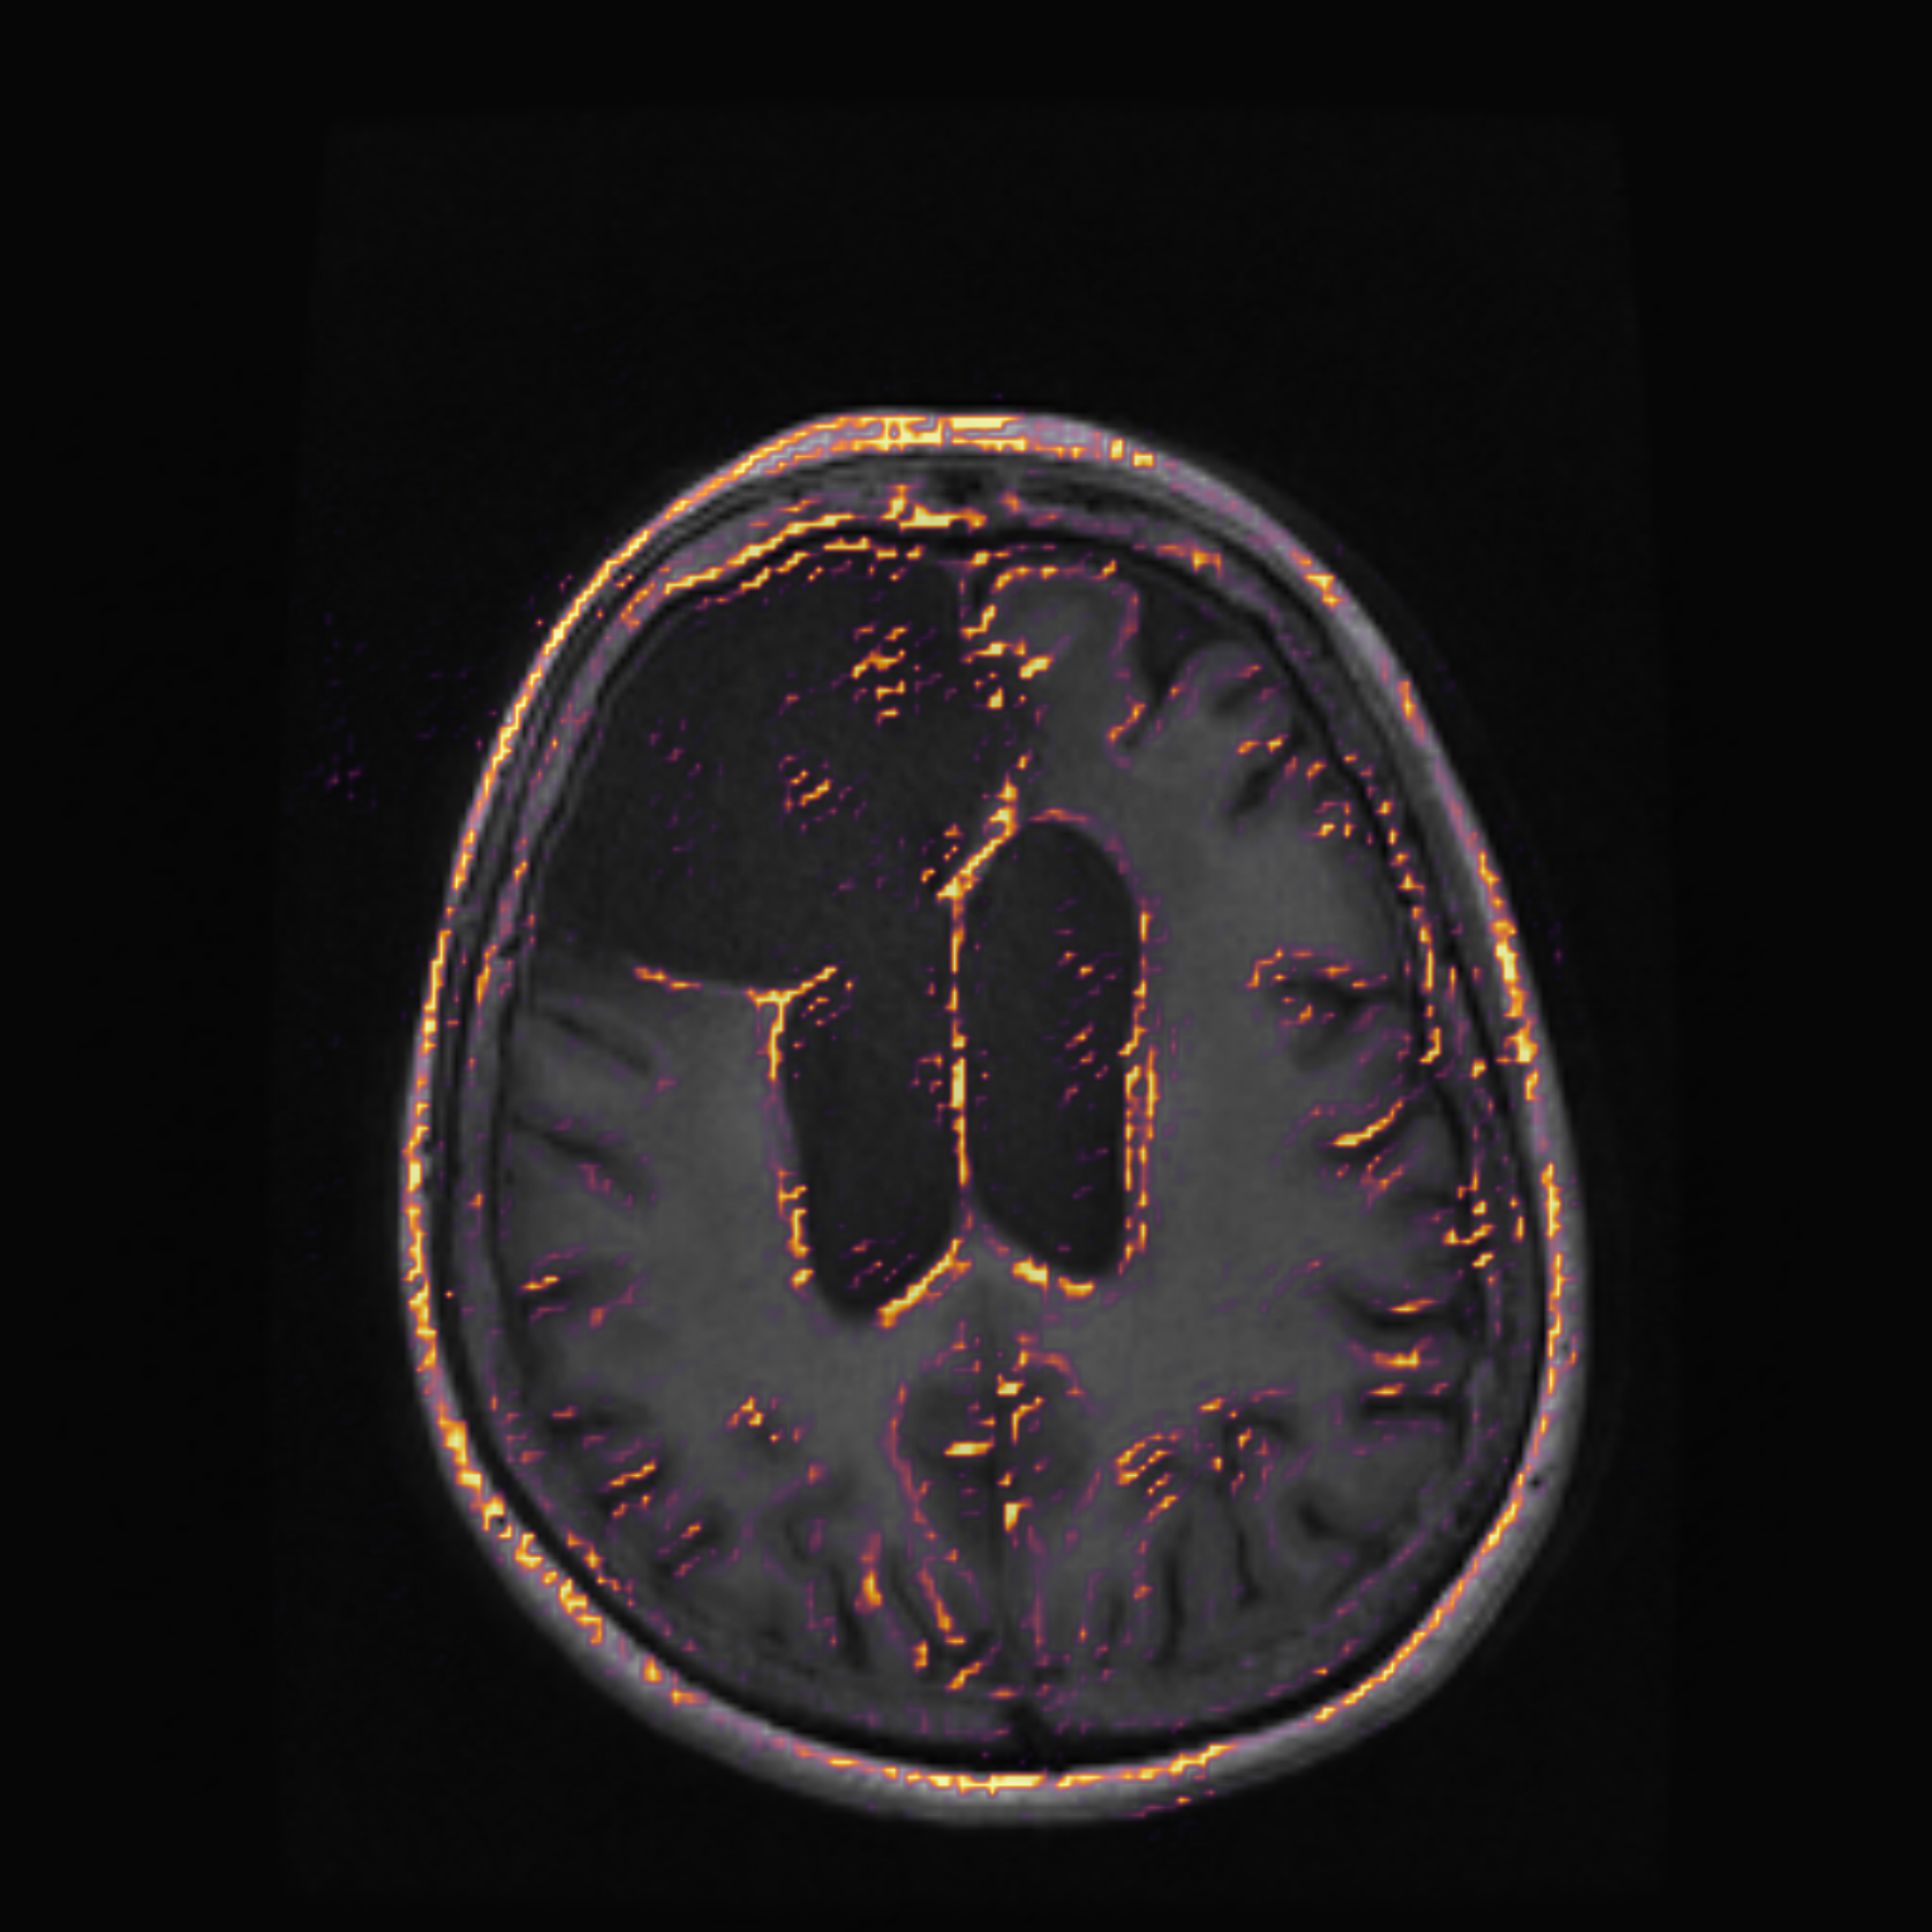
\includegraphics[width=\textwidth]{Figures/T1_saliency}
        \caption{\gls{T1}}\label{fig:T1Cam}
    \end{subfigure}
    \begin{subfigure}[t]{\figexamplewidth}
        \centering
        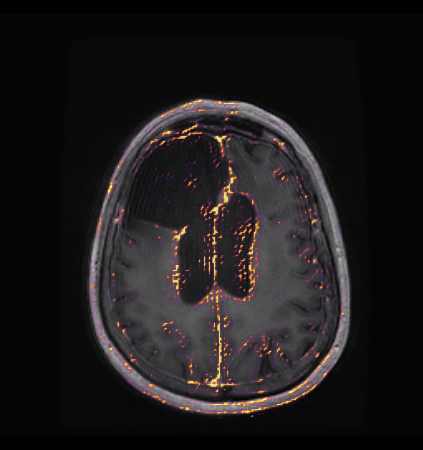
\includegraphics[width=\textwidth]{Figures/T1GD_saliency}
        \caption{\gls{T1C}}\label{fig:T1GDCam}
    \end{subfigure}
    \begin{subfigure}[t]{\figexamplewidth}
        \centering
        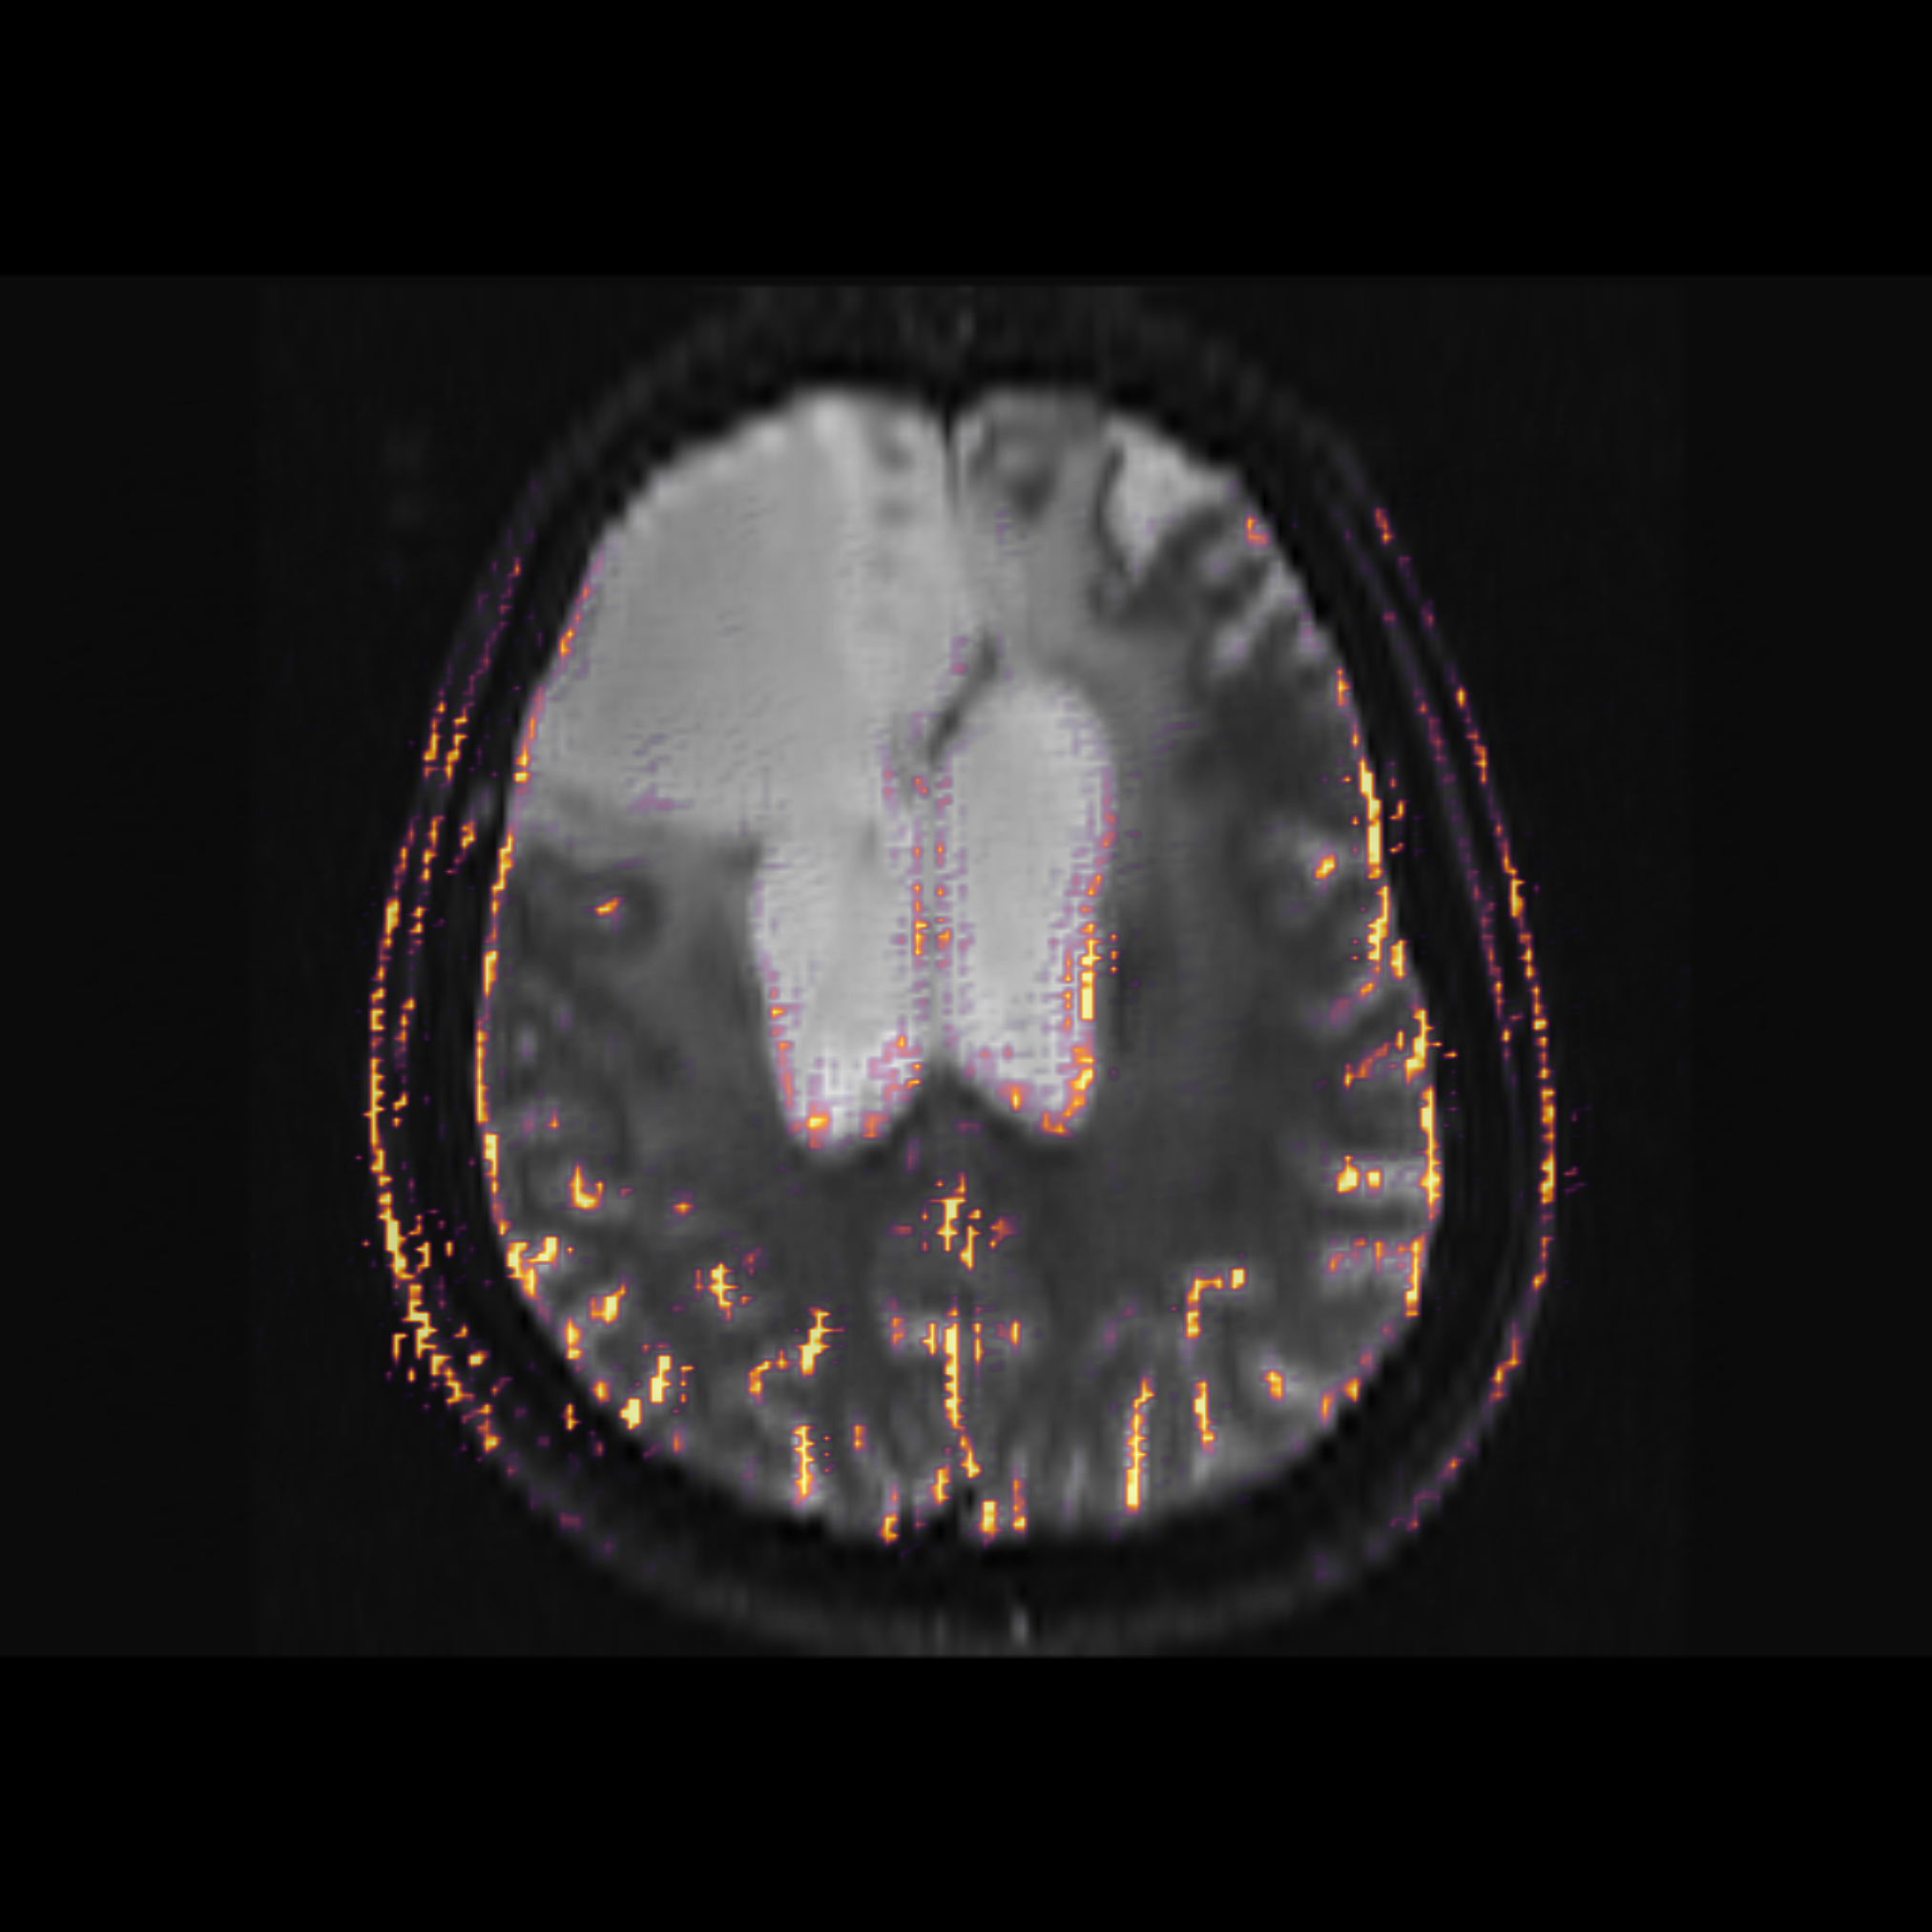
\includegraphics[width=\textwidth]{Figures/T2_saliency}
        \caption{\gls{T2}}\label{fig:T2wCam}
    \end{subfigure}
    \begin{subfigure}[t]{\figexamplewidth}
        \centering
        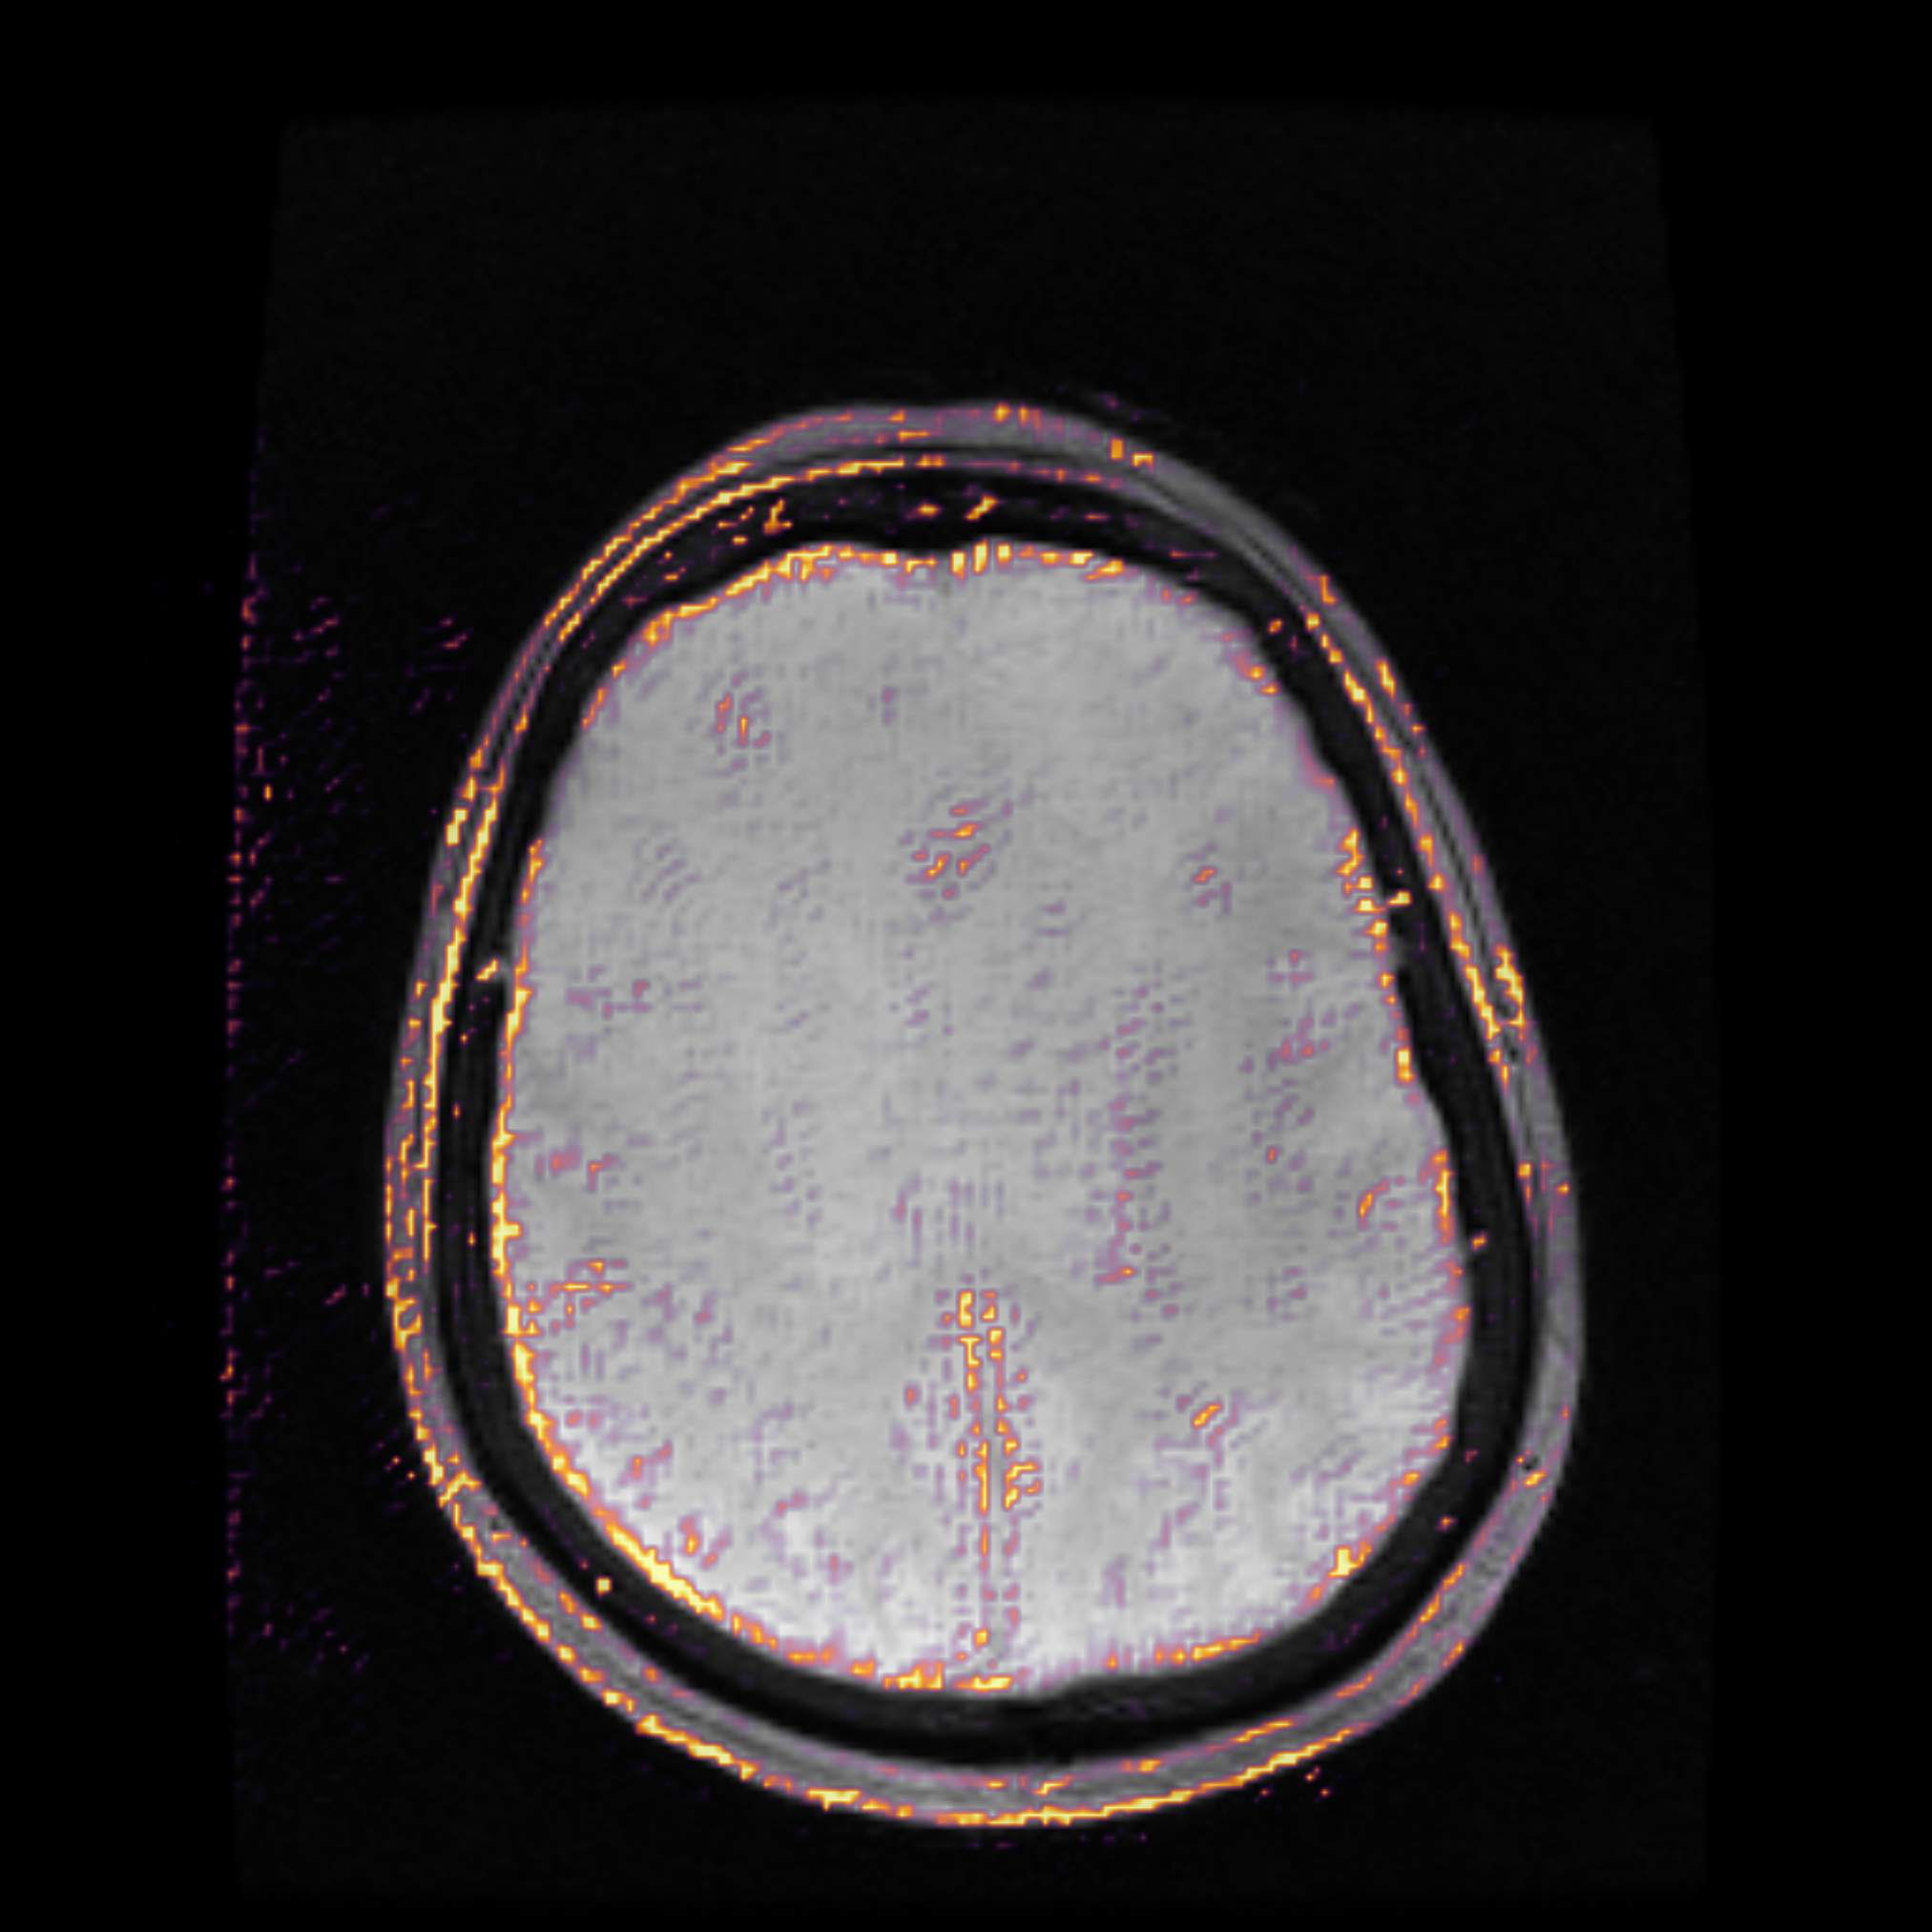
\includegraphics[width=\textwidth]{Figures/PD_saliency}
        \caption{\gls{PD}}\label{fig:PDwCam}
    \end{subfigure}


    \begin{subfigure}[t]{\figexamplewidth}
        \centering
        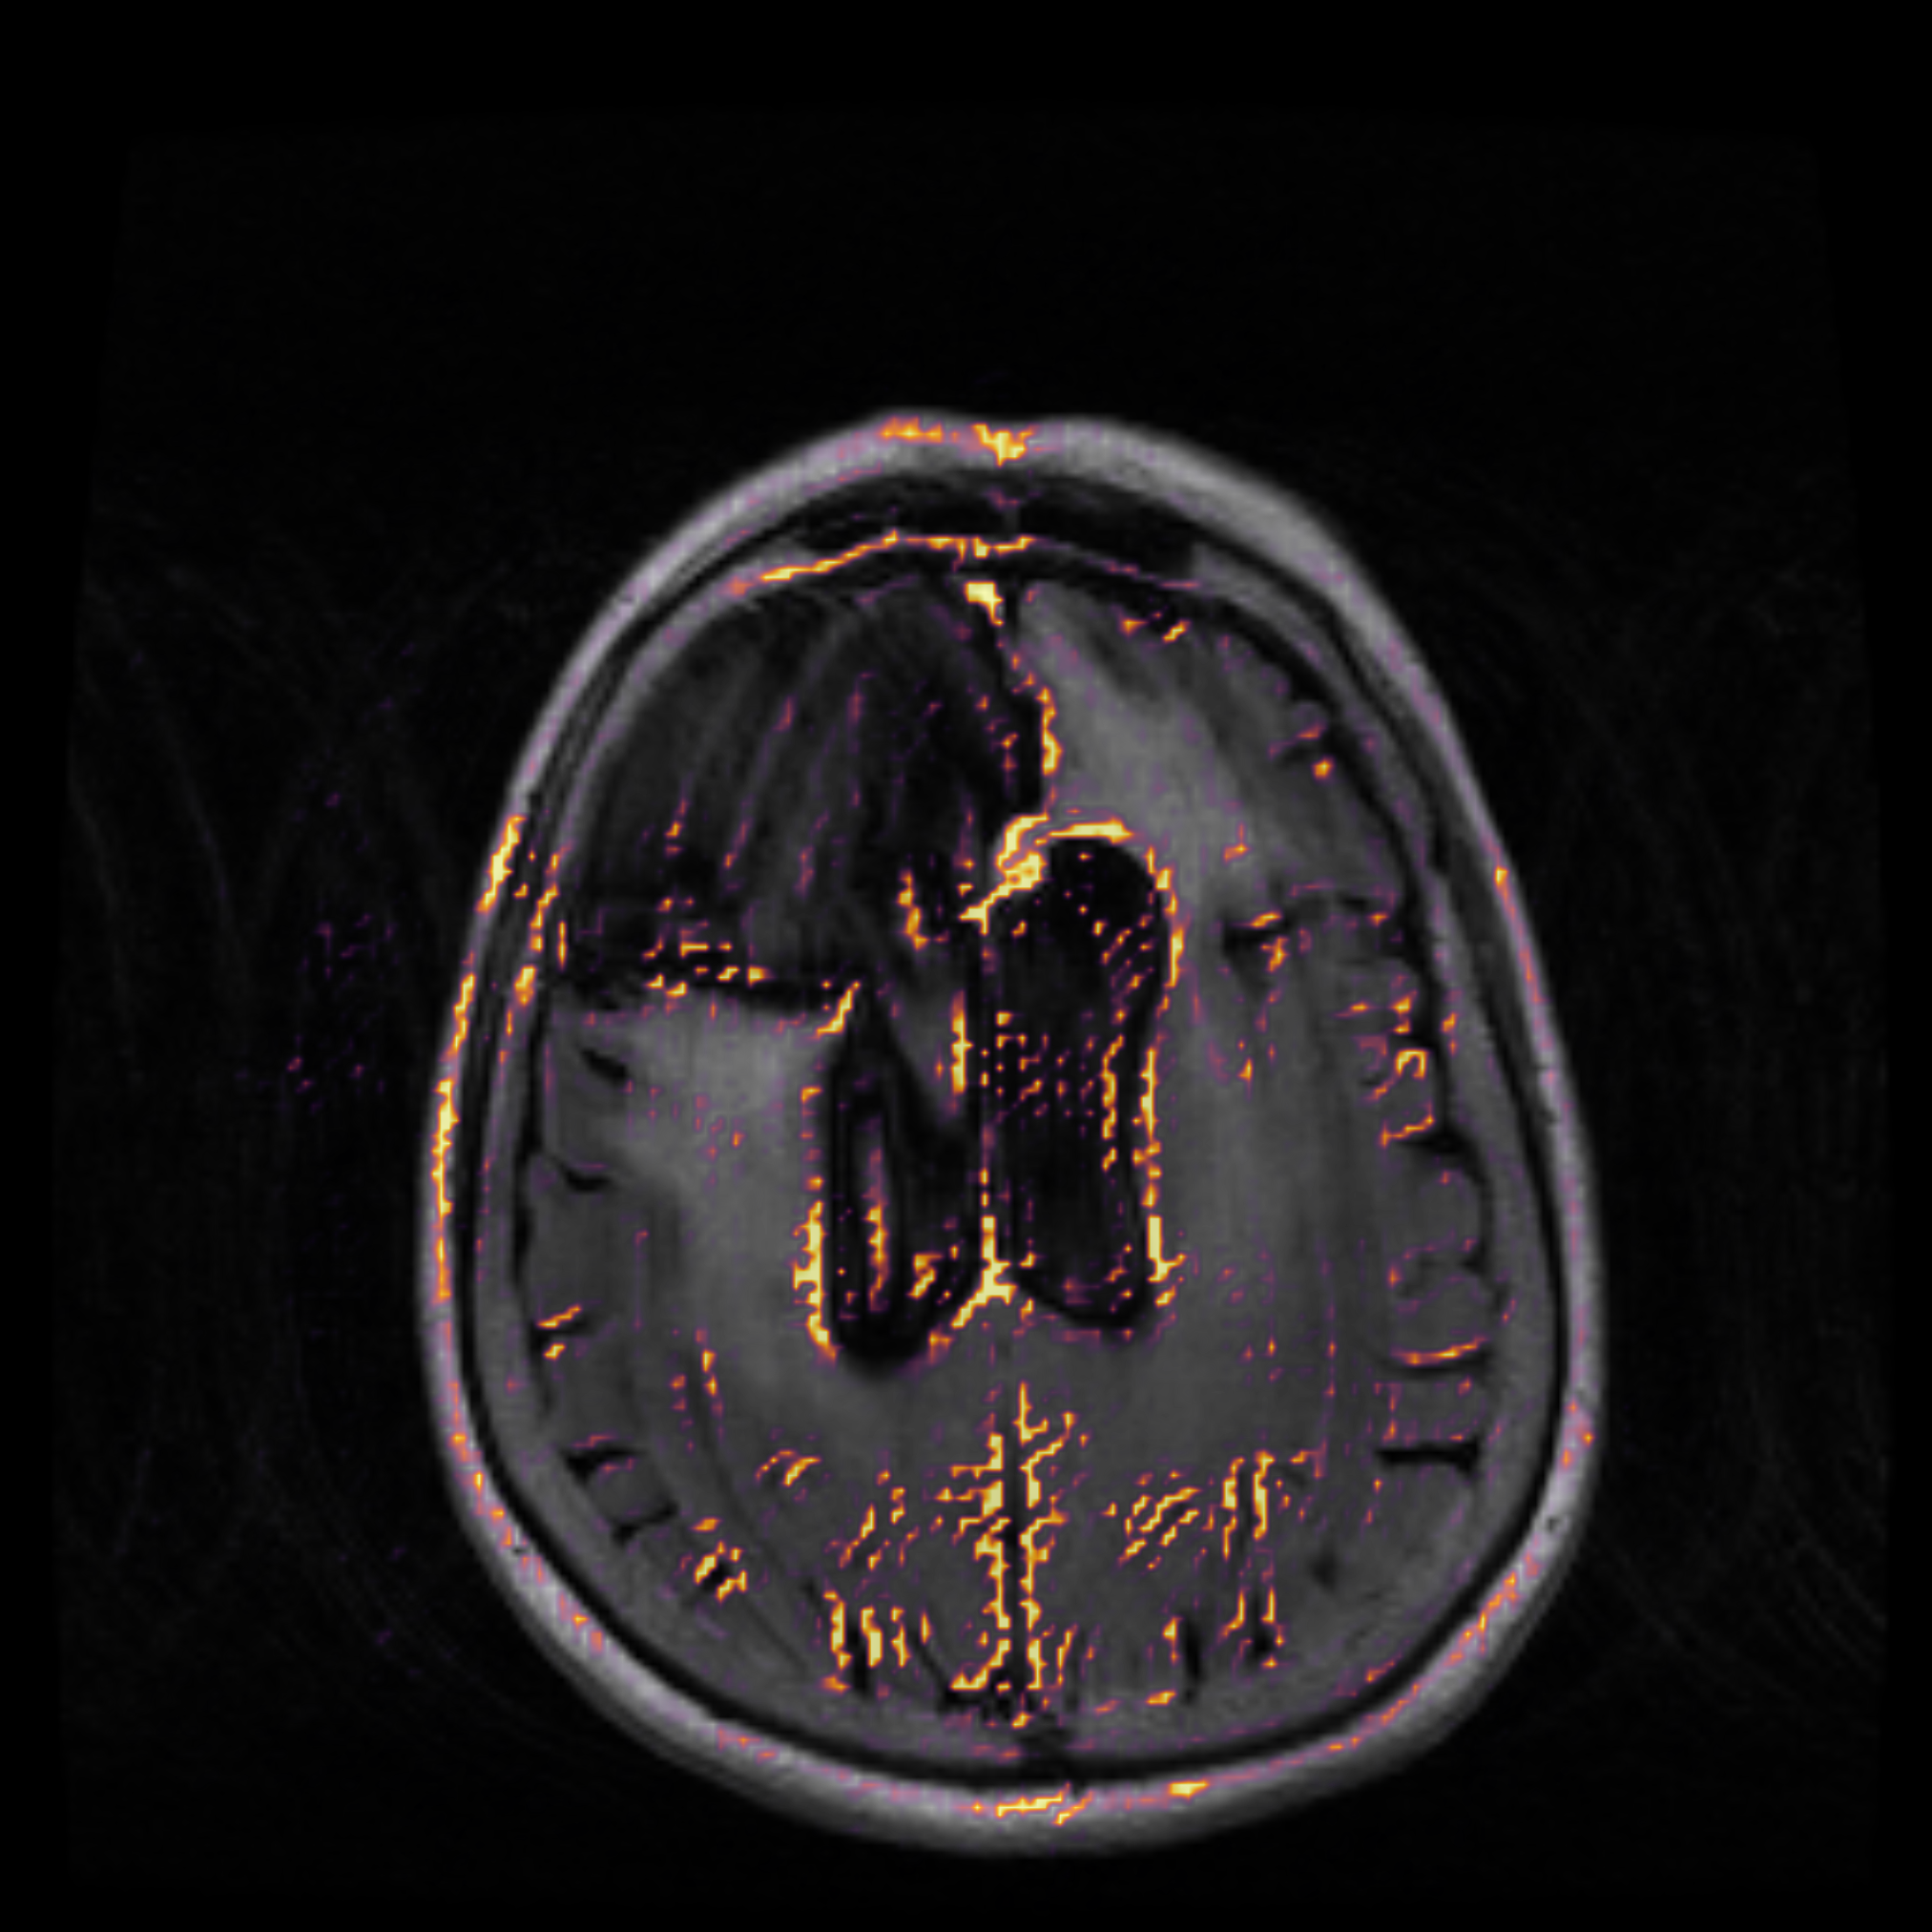
\includegraphics[width=\textwidth]{Figures/FLAIR_saliency}
        \caption{\gls{FLAIR}}\label{fig:FLAIRCam}
    \end{subfigure}
    \begin{subfigure}[t]{\figexamplewidth}
        \centering
        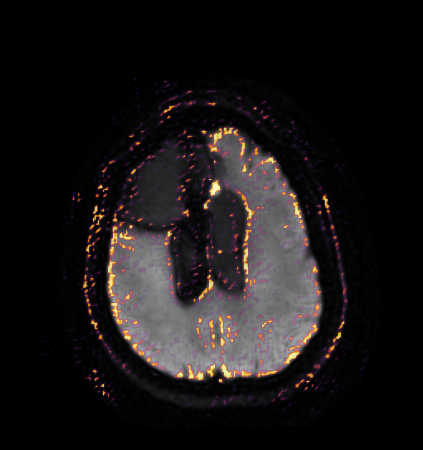
\includegraphics[width=\textwidth]{Figures/DWI_saliency}
        \caption{\gls{DWI}}\label{fig:DWICam}
    \end{subfigure}
    \begin{subfigure}[t]{\figexamplewidth}
        \centering
        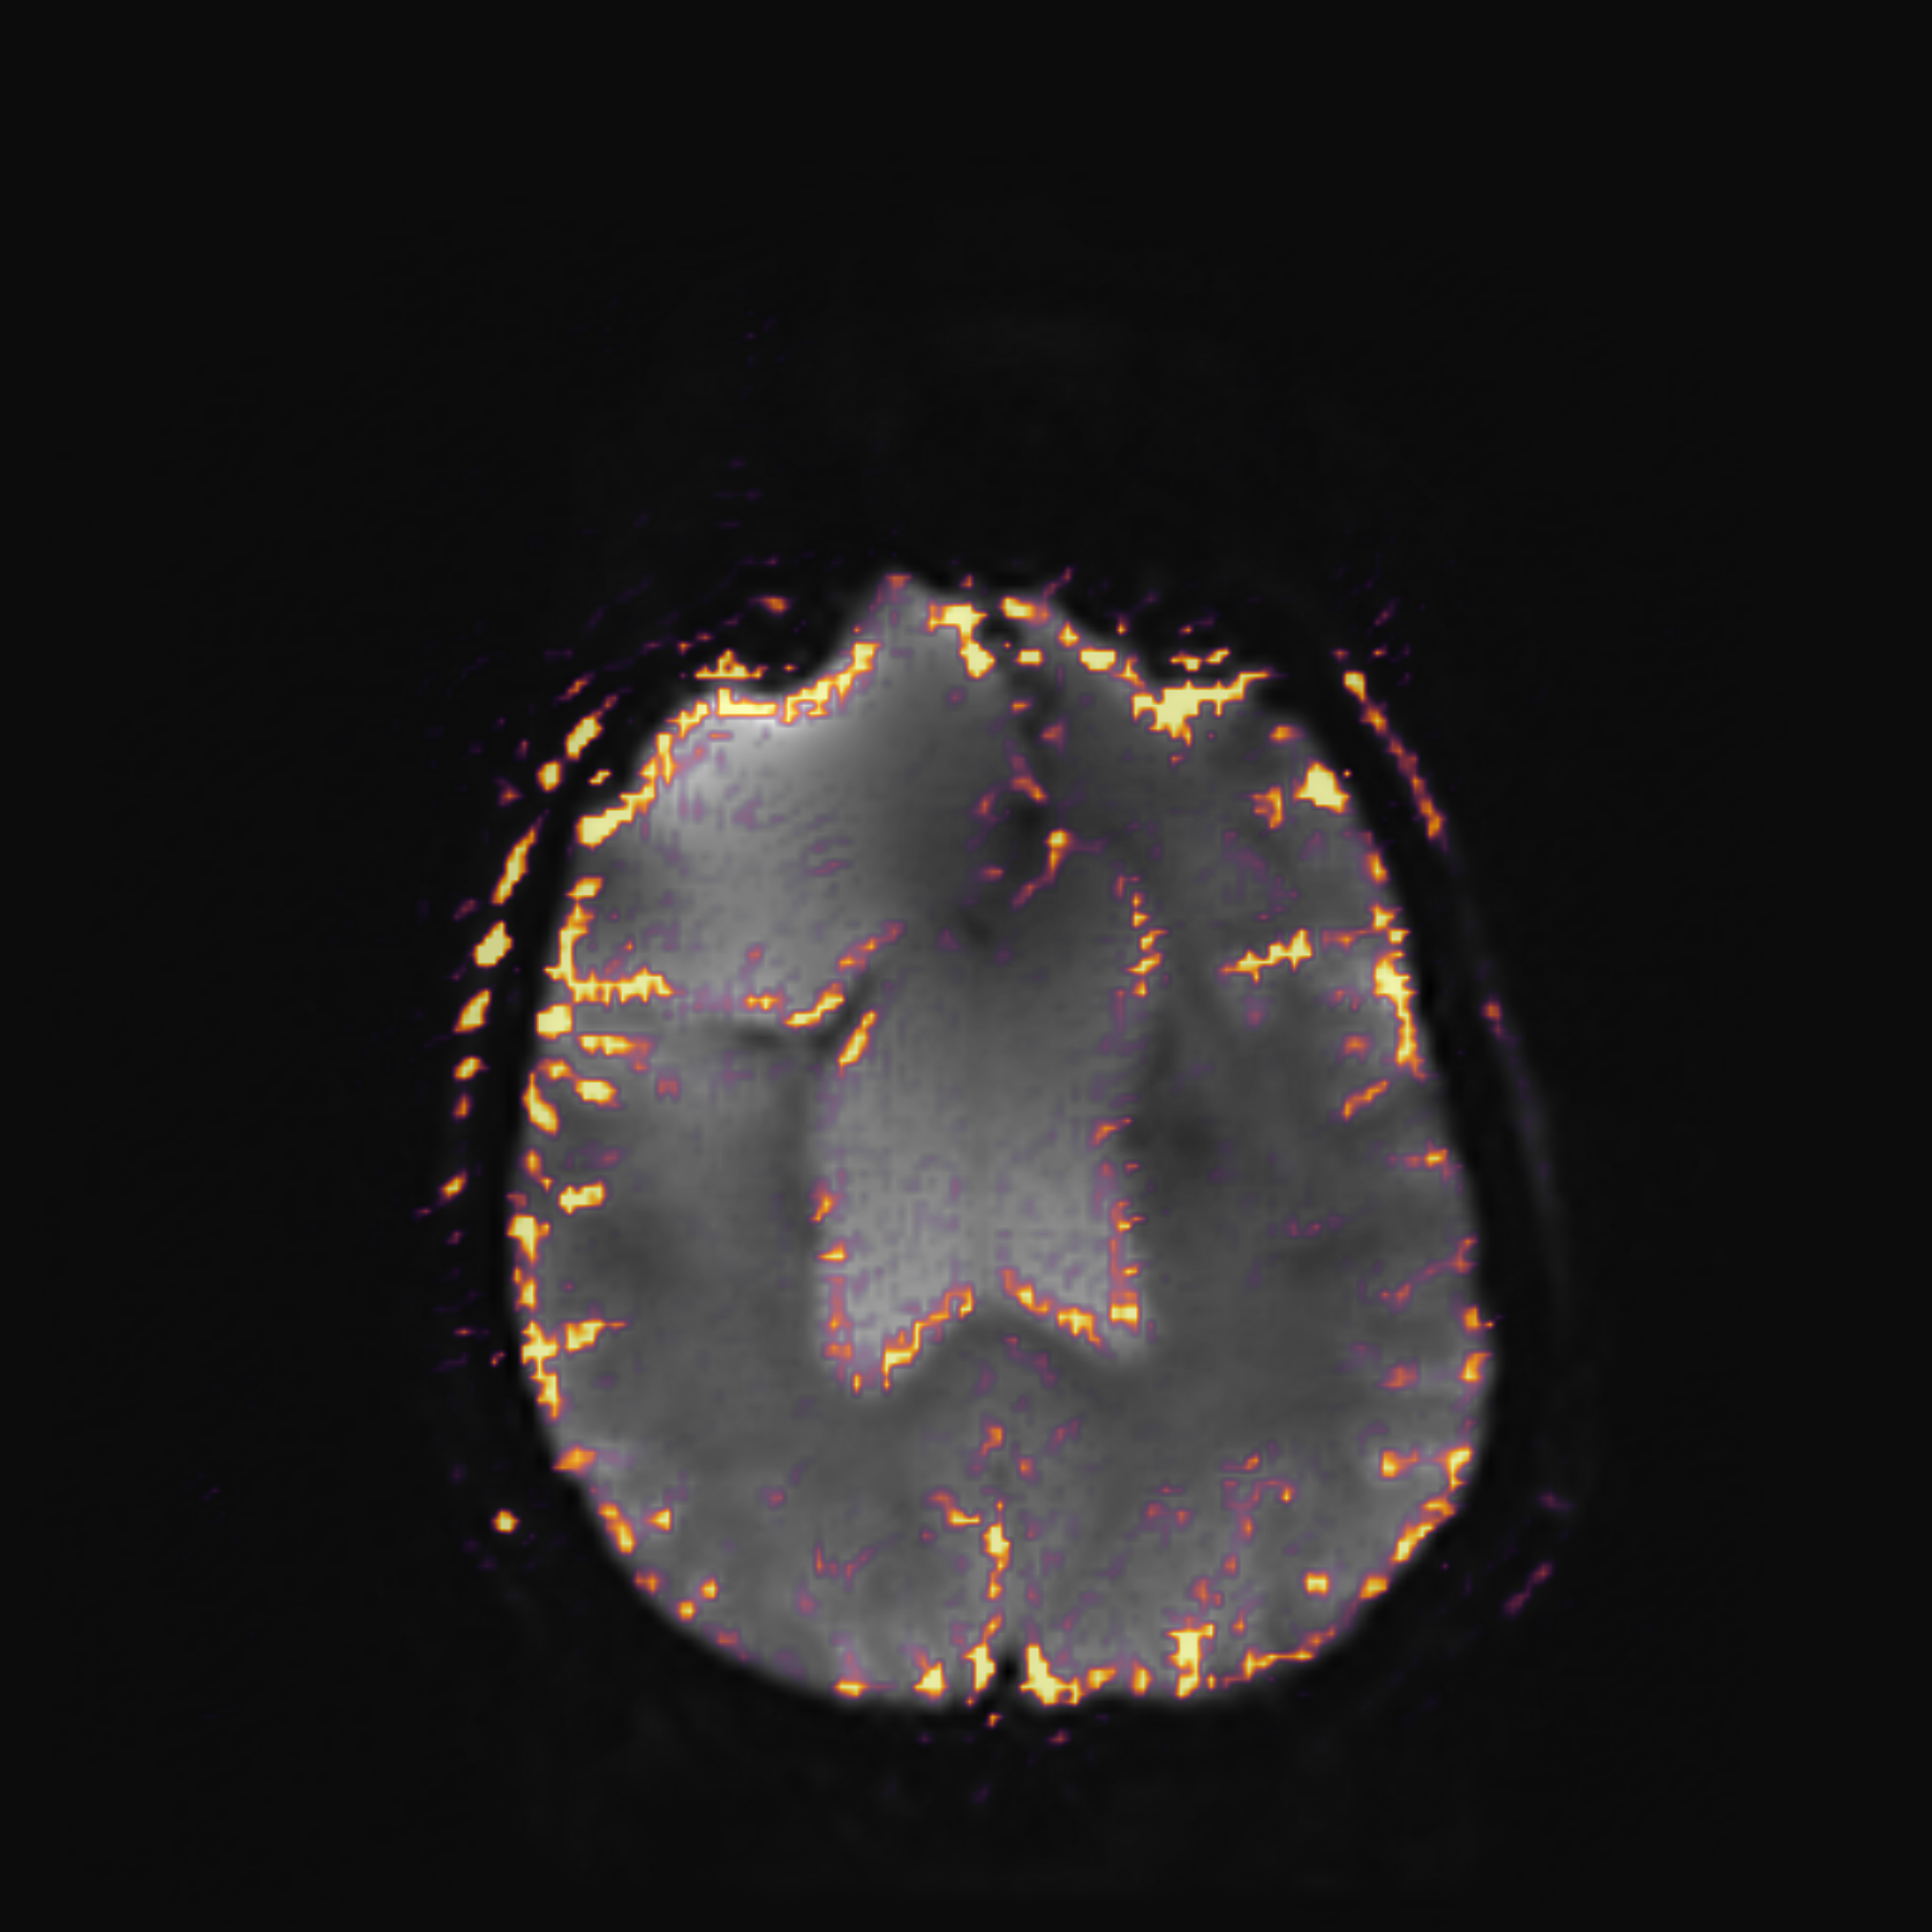
\includegraphics[width=\textwidth]{Figures/DSC_saliency}
        \caption{\gls{DSC}}\label{fig:PWICam}
    \end{subfigure}
    \begin{subfigure}[t]{\figexamplewidth}
        \centering
        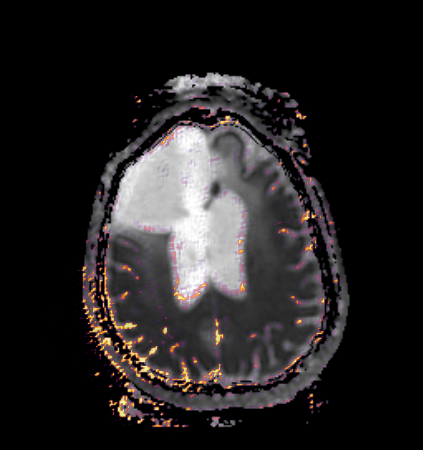
\includegraphics[width=\textwidth]{Figures/DERIVED_saliency}
        \caption{Derived (ADC)}\label{fig:DWI-DCam}
    \end{subfigure}
    \caption{Saliency maps of the \glspl{type}, generated by the \gls{CNN} evaluated on the same \glspl{slice} as in \cref{fig:seq_examples}. This \gls{CNN} was the model obtained in Experiment I}\label{fig:seq_gradcam}
\end{figure}

\subsection{\acrlong{HC} predictive performance}

The top-level rules of the  derived heuristic for \gls{HC} were mainly based on the series description, with additional lower-level rules based on the echo time, image type, and the derived status of the \gls{scan}.
The overall accuracy obtained within the \gls{BTtrain} after several iterations of improving the heuristic was \per{91.0}.
The overall accuracy in the \gls{BTtest} was \per{72.0}.
The results for each \gls{class} can be found in \cref{tab:heudiresults}, along with a comparison to the accuracy of the \gls{CNN} evaluated on the \gls{BTtest}.
For the evaluation of the \gls{CNN}'s performance, we included the same \glspl{scan} as present in the test set for \gls{HC} (i.e. those which were available in \gls{DICOM} format).
Although a slightly different \gls{ds} was used for this test set, the results of the \gls{CNN} in \cref{tab:seqacc} and \cref{tab:heudiresults} appear to be the same.
This can be explained by the fact that only \gls{T1C} \glspl{scan} were removed from the test set, thus for all other \glspl{class} the accuracy remained the same.
Furthermore, due to the large number of \glspl{scan} the difference is only visible at more decimals, e.g. the overall accuracy in \cref{tab:seqacc} was \per{98.73} whereas in \cref{tab:heudiresults} it was \per{98.72}.
These results show that \gls{DDS} outperformed \gls{HC} both in terms of the overall accuracy and the per-class accuracy for all \glspl{class}.
\cref{app:timing} compares the time required to sort the \glspl{ds} using either \gls{DDS}, \gls{HC}, or by hand, which shows that \gls{DDS} is more than twice as fast as the other two methods.

\begin{table}[htbp]

 \centering
  \begin{tabular}{lS[table-format=1.3]S[table-format=1.3]}
      \toprule

  & {\textbf{\acrlong{HC}}} & {\textbf{\acrlong{DDS}}}\\
  \midrule
  Overall   & 0.720 & 0.987\\
  \cmidrule{2-3}
  \acrshort{T1}       & 0.963 & 0.993\\
  \acrshort{T1C}      & 0.447 & 0.997\\
  \acrshort{T2}       & 0.930 & 0.990\\
  \acrshort{PD}       & 0.077 & 1.000\\
  \acrshort{FLAIR} & 0.684 & 0.930\\
  \acrshort{DWI}       & 0.887 & 0.991\\
  \acrshort{DSC}   & 0.600 & 1.000\\
  Derived   & 0.948 & 0.994\\
  \bottomrule
  \end{tabular}
  \caption{Accuracy of \acrlong{HC} on the \gls{BTtest}. Results of \gls{DDS} on this test set are also given, where the \glspl{scan} which were not available in the \gls{DICOM} format were excluded from the test set}\label{tab:heudiresults}

\end{table}


\section{Discussion}
\label{sec:discussion}
Our results show that it is possible to use a \gls{CNN} to automatically identify the \gls{type} of brain \gls{MRI} \glspl{scan} and use this to sort a large, heterogeneous \gls{ds}.
Because of the high accuracy of our method, it can be used virtually without manual verification.
The \gls{CNN} performed well both for \glspl{scan} with and without the presence of a \gls{tumor}.
The performance of our method generalizes well across \glspl{scan} from different \glspl{site}, scanners, \glspl{sub}, and scan protocols.
Our method was also able to correctly predict the \gls{type} of \glspl{scan} that had poor imaging quality or contained imaging artifacts, as can be seen in \cref{app:randomtumorsample}.
The \gls{CNN} focused mainly on the ventricles, areas close to the skull, and the \gls{CSF} at the edges of the brain.
There was also some focus on the gray matter and white matter, although these structures seemed less relevant for the decision making of the \gls{CNN}.
It makes sense that the \gls{CNN} focuses on the \gls{CSF}, both in the ventricles and at the edges of the brain, because their visual appearance is very characteristic of the \gls{type}.
Although the \gls{CNN} also focused on the eyes and nose, we do not expect this to disrupt the prediction when these structures are absent (e.g. in defaced \glspl{scan}).
There were a lot of \glspl{slice} in which the eyes and nose were not present, such as the most inferiorly and superiorly located \glspl{slice}, for which the \gls{CNN} predicted the \gls{type} correctly.

Data sorting is just one step of the data curation pipeline, and in recent years more research on the automation of other data curation tasks has been carried out.
Some examples include automatic \gls{scan} quality checking \autocite{esteban2017mriqc}, motion artifact correction \autocite{tamada2020motion}, and missing \gls{type} imputation from the present \glspl{type} \autocite{lee2019collagan}.
However, to automate other data curation steps the \gls{ds} first needs to follow a structured format, making our tool a crucial first step in the overall pipeline.
The increasing data complexity, both in volume and in the number of different types of data, not only shows a need for a proper data curation pipeline, but also shows the need for a standardized data structure for \glspl{scan} and their associated metadata \autocite{erp2011infrastructure, gorgolewski2016brain, lambin2017radiomics}.
The widespread adoption of a common, standardized data structure would be favorable over the use of our tool or similar tools.
Unfortunately, both in research and in clinic practice, it is currently not commonplace to provide \glspl{ds} in a standardized format, thus making our tool a valuable addition to the data curation pipeline.
Even if a standardized data structure were to be widely adopted, our tool would remain valuable as a quality assessment tool.

Although the accuracy of our method is high overall, our method predicted the incorrect \gls{type} in some cases.
For example, in Experiment I the \gls{CNN} mainly misclassified \gls{FLAIR} \glspl{scan}.
Almost all of these misclassified \gls{FLAIR} \glspl{scan} originated from the \gls{RIDER} \gls{ds}.
Comparing a \gls{FLAIR} \gls{scan} from the \gls{RIDER} \gls{ds} with a \gls{FLAIR} \gls{scan} from the train set used in Experiment I shows a  big difference in visual appearance, see \cref{fig:IvyGAP_FLAIR} and \cref{fig:RIDER_FLAIR}.
These figures show that the white matter and gray matter appear very different on the two \glspl{scan}, even though they have the same \gls{type}, which probably confused the network.
In Experiment II the per-class accuracy was the lowest for the \gls{T2} \glspl{scan}.
Almost all of the misclassified \gls{T2} \glspl{scan} were hippocampus \glspl{scan}, an example of which can be seen in \cref{fig:T2_hippo}.
The misclassification of these \glspl{scan} can be explained by their limited field of view.
Since the \gls{CNN} did not see any such \glspl{scan} in the training set, as all \glspl{scan} in the training set covered the full brain, it is not surprising that our method failed in these cases.
The saliency maps in \cref{fig:FLAIR_comparison} show that the \gls{CNN} had difficulty focusing on the relevant parts of the \gls{slice}.
For example, for the \gls{FLAIR} \glspl{slice} in \cref{fig:FLAIRCam} and \cref{fig:IvyGAP_FLAIR_saliency} it can be seen that the \gls{CNN} focused mainly on the ventricles, whereas in \cref{fig:RIDER_FLAIR_saliency} there was more focus on the edge of the brain, similar to \gls{T1} \gls{slice} in \cref{fig:T1Cam}.
Although we did not achieve a perfect prediction accuracy, it is unlikely that any \gls{scan} sorting method ever will, due to the large heterogeneity in \gls{scan} appearance and \gls{scan} metadata.
While not perfect, our method does have a very high performance overall and the comparison with manual sorting shows that it considerably reduces the time required to sort a \gls{ds}.

The \gls{CNN} was trained and evaluated by using the ground truth labels, which were obtained by manually going through the dataset and annotating each \gls{scan} according to the perceived \gls{type}.
It is possible that the \gls{type} was incorrectly annotated for some of the \glspl{scan}.
To limit this possibility we took a second look at \glspl{scan} where there was a mismatch between the prediction from \gls{DDS} and the ground truth label, both for train \glspl{ds} and test \glspl{ds}.
We corrected the ground truth label for \glspl{scan} that were incorrectly annotated and these corrected labels were used for the experiments presented in this paper.
The labels of around \per{0.1} of the \glspl{scan} in the \gls{ds} were corrected in this way.
Although it is possible that there were still some incorrectly annotated \glspl{scan}, based on these findings we expect this fraction to be very small.

\begin{figure}
\centering
    \begin{subfigure}[t]{0.25\textwidth}
        \centering
        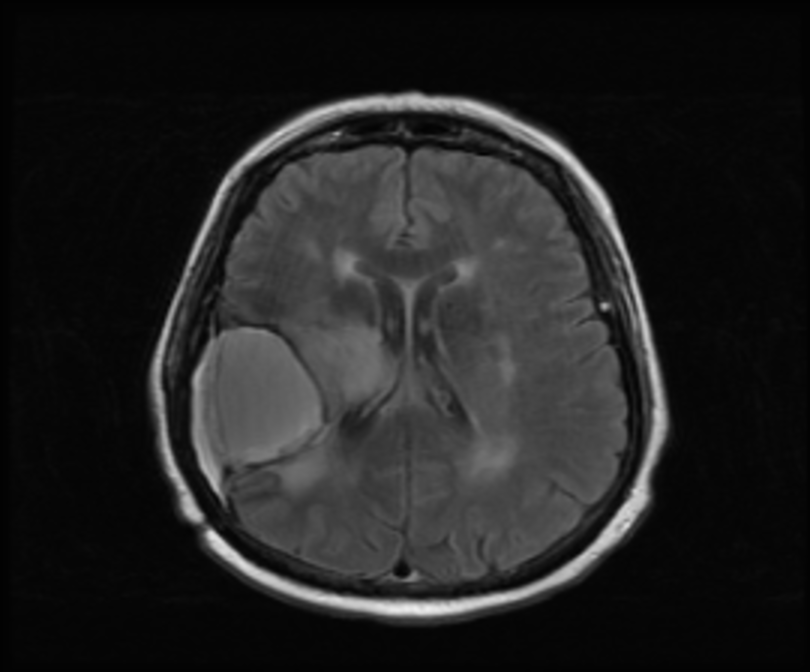
\includegraphics[width=\textwidth]{Figures/FLAIR_Ivy}
        \caption{\gls{FLAIR} \gls{scan} from the \gls{IVY} collection. This \gls{type} was correctly predicted}\label{fig:IvyGAP_FLAIR}
    \end{subfigure}
    \hfill
    \begin{subfigure}[t]{0.25\textwidth}
        \centering
        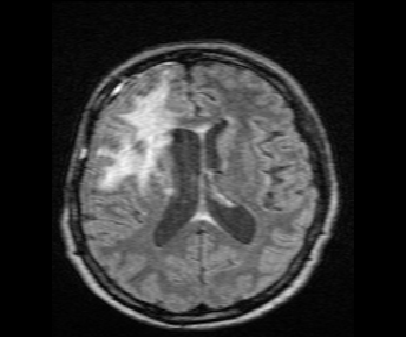
\includegraphics[width=\textwidth]{Figures/FLAIR_RIDER}
        \caption{\gls{FLAIR} \gls{scan} from the \gls{RIDER} collection. This \gls{type} was misclassified as a \gls{T1}}\label{fig:RIDER_FLAIR}
    \end{subfigure}
    \hfill
    \begin{subfigure}[t]{0.25\textwidth}
        \centering
        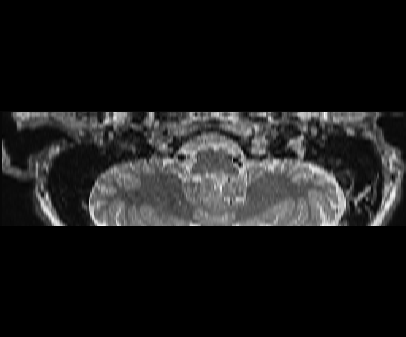
\includegraphics[width=\textwidth]{Figures/T2_hippocampus}
        \caption{\gls{T2} \gls{scan} from the \gls{NTTS}. This \gls{type} was misclassified as a \gls{T1C}}\label{fig:T2_hippo}
    \end{subfigure}

    \begin{subfigure}[t]{0.25\textwidth}
        \centering
        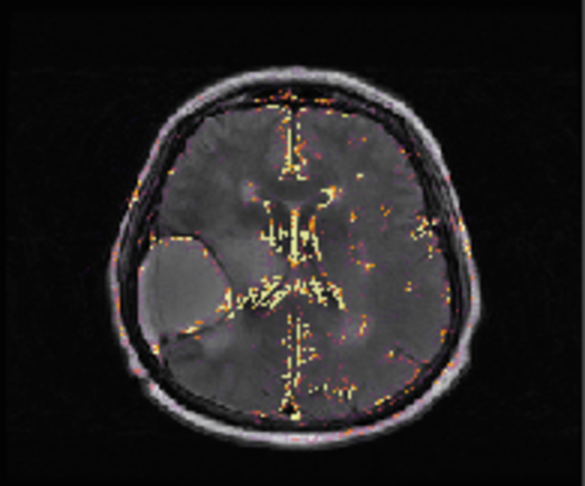
\includegraphics[width=\textwidth]{Figures/FLAIR_Ivy_Saliency}
        \caption{Saliency map of the correctly classified \gls{scan} from \protect\subref{fig:IvyGAP_FLAIR}}\label{fig:IvyGAP_FLAIR_saliency}
    \end{subfigure}
    \hfill
    \begin{subfigure}[t]{0.25\textwidth}
        \centering
        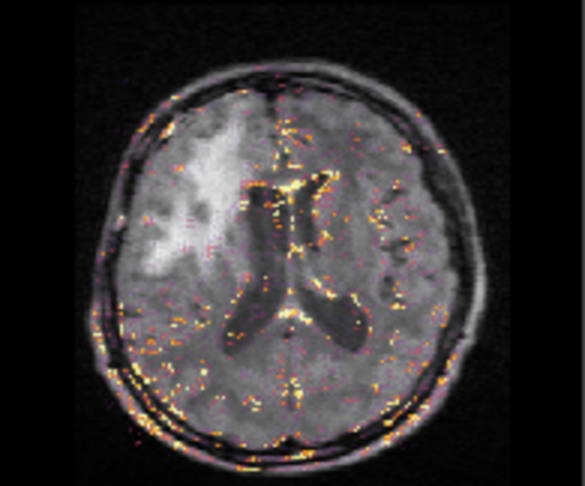
\includegraphics[width=\textwidth]{Figures/Appendix/FLAIR_RIDER_saliency}
        \caption{Saliency map of the misclassified \gls{scan} from \protect\subref{fig:RIDER_FLAIR}}\label{fig:RIDER_FLAIR_saliency}
    \end{subfigure}
    \hfill
    \begin{subfigure}[t]{0.25\textwidth}
        \centering
        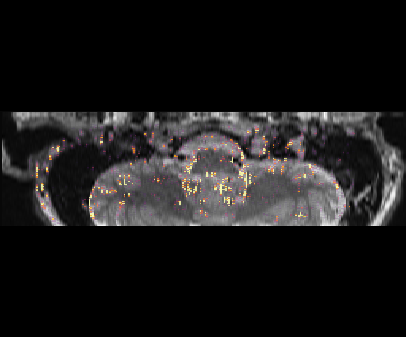
\includegraphics[width=\textwidth]{Figures/Appendix/Saliency_T2_hippo.pdf}
        \caption{Saliency map of the misclassified \gls{scan} from \protect\subref{fig:T2_hippo}}\label{fig:T2_hippo_saliency}
    \end{subfigure}

\caption{Examples of \glspl{scan} our method misclassified (\protect\subref{fig:RIDER_FLAIR} and \protect\subref{fig:T2_hippo}) and a correctly classified \gls{scan} \protect\subref{fig:IvyGAP_FLAIR} as comparison, along with their saliency maps.
The \gls{FLAIR} \gls{scan} in \protect\subref{fig:RIDER_FLAIR} is probably misclassified as its appearance is very different from \gls{FLAIR} \glspl{scan} that were in the train \gls{ds}.
The \gls{T2} \gls{scan} in \protect\subref{fig:T2_hippo} is probably misclassified because it has a very limited field of view}
\label{fig:FLAIR_comparison}

\end{figure}

We chose a \gls{CNN} as the basis of our method because we wanted to minimize the number of pre-processing steps.
Using more traditional machine learning approaches, such as a support vector machine or random forest, would require the extraction of relevant features from each \gls{scan}.
This would complicate our method as we would first have to hand-craft these features and add a pre-processing step in which we extract these features from the \gls{scan}.
Furthermore, the extraction of these features would likely require a brain mask to prevent the features from being influenced too much by the background.
The creation of this brain mask would add a pre-processing step, and could be a potential source of error.
Instead, by using a \gls{CNN}, no features had to be defined as the \gls{CNN} automatically learns the relevant features.
The \gls{CNN} also does not require a brain mask, as it has learned to ignore the background and focus on the brain itself, as shown by the saliency maps.

We opted for a 2D \gls{CNN} instead of a 3D \gls{CNN}, because this allowed us to extract a larger region of the \gls{scan} to be used as an input for the \gls{CNN}.
By using a 2D \gls{CNN}, this region could encompass a full slice of the brain enabling the \gls{CNN} to learn features that capture the relative differences in appearance of the various tissue types (white matter, gray matter, \acrshort{CSF}, bone, skin, etc.), which are characteristic of the \gls{type}.
Furthermore, because a 2D \gls{CNN} typically requires less memory than a 3D \gls{CNN} \autocite{prasoon2013deep}, it requires less computational power (making our method accessible to a broader audience), and also requires less time to train and evaluate \autocite{rongjian2014deep}.

Our method achieved a better overall accuracy and per-class accuracy than \gls{HC}.
The results obtained using \gls{HC} show the difficulty of creating a method based on \gls{DICOM} tags that generalizes well to other \glspl{ds}.
Even within one dataset, it can be difficult to create a heuristic that correctly maps the \gls{scan} metadata to the \gls{type}; for example \cref{tab:heuditags}, shows that 1215 different series descriptions are used just for the eight \glspl{type} considered in this research.
\gls{HC} has particular difficulty in identifying \glspl{scan} that have similar metadata but have different \glspl{type}.
For example, this is reflected in the results for the \gls{T1} and \gls{T1C} \glspl{scan}.
These \glspl{scan} usually have similar scan settings and series descriptions, making it hard to determine whether a \gls{scan} is obtained pre- or post-contrast administration.
The same difficulty plays a role for \gls{T2} and \gls{PD} \glspl{scan}, which are often acquired at the same time in a combined imaging sequence and thus have the same series description.
In our timing results (\cref{app:timing}), it was faster to sort the \gls{ds} by hand than to use \gls{HC}.
This was caused by \gls{HC} often misclassifying \gls{FLAIR} and \gls{T1C} \glspl{scan} as a different \gls{type}, and thus a lot of manual time was needed to correct these mistakes.

A method that, similar to ours, classifies the \gls{type} based on the visual appearance of the \gls{scan} was proposed by~\autocite{remedios2018classifying} called $\Phi$-net.
Their method can identify \gls{T1}, \gls{T1C}, \gls{T2}, and pre-contrast and post-contrast FLAIR \glspl{scan}.
\citeauthorref{remedios2018classifying} do this using a cascaded \gls{CNN} approach where a first \gls{CNN} is used to classify a \gls{scan} as T1-weighted, T2-weighted, or FLAIR.
Two other \glspl{CNN} are then used to classify a \gls{scan} as pre-contrast or post-contrast, one \gls{CNN} for the T1-weighted \glspl{scan} and one \gls{CNN} for the FLAIR \glspl{scan}.
$\Phi$-net achieved an overall accuracy of \per{97.6}, which is lower than our overall accuracy of \per{98.7} (Experiment I) and \per{98.5} (Experiment II).
Since \citeauthorref{remedios2018classifying} did not make their trained model publicly available, it was not possible to directly compare performances on the same \gls{ds}.
\citeauthorref{remedios2018classifying} tested their method on 1281 \glspl{scan}, which came from 4 different \glspl{site} and 5 different scanner models.
Their \gls{ds} was thus considerably smaller and less heterogeneous than our test data set.
Furthermore, our method can identify more \glspl{type} and does so using only a single \gls{CNN} instead of three.

A limitation of our method is that it can only classify a \gls{scan} as one of the eight \glspl{type} for which it was trained.
Thus, when it is presented with an unknown \gls{type} (e.g. \gls{ASL} or dynamic contrast-enhanced perfusion-weighted imaging), our method will (wrongly) predict it as one of the other \glspl{class}.
In future work, this limitation could be addressed in two ways.
The first option would be to adapt the network to either recognize more \glspl{type} or to replace one of the existing \glspl{class} by a different one.
This can be done using a transfer learning approach by fine-tuning the weights obtained in this research on additional data \autocite{tajbakhsh2016convolutional}.
Since we did not have enough data for other \glspl{type}, we limited the \gls{CNN} to the eight \glspl{class} for which we did have enough data.
A second option would be to extend our method to allow out-of-distribution detection \autocite{devries2018learning}.
In this methodology, the network could not only predict the \gls{type} of a \gls{scan} but could also indicate if a \gls{scan} belongs to an unknown \gls{type}.
This requires a significant change to the model architecture, which we considered outside the scope of this research for now.

Another limitation is the use of reorient2std from FSL, which means that (this part of) the code cannot be used in a commercial setting.
Commercially allowed alternatives exist, such as the \say{reorient\_image} function from ANTs (\url{http://stnava.github.io/ANTs/}), however these have not been tested as part of the \gls{DDS} pipeline.

A promising future direction could be to predict the metadata of a \gls{scan} based on its visual appearance.
For example, one could predict the sequence that has been used to acquire a \gls{scan} (e.g. MPRAGE or MP2RAGE in the case of a \gls{T1} \gls{scan}), or reconstruct the acquisition settings of a \gls{scan} (e.g. the spin echo time).
In this research, we did not consider these types of predictions because we first wanted to focus on the \gls{ds} organization, however we think that our method can provide a basis for these types of predictions.

\section{Conclusion}

We developed an algorithm that can recognize \gls{T1}, \gls{T1C}, \gls{T2}, \gls{PD}, \gls{FLAIR}, \gls{DWI}, \gls{DSC}, and derived brain \gls{MRI} \glspl{scan} with high accuracy, outperforming the currently available methods.
We have made our code and trained models publicly available under an Apache 2.0 license\footnote{\url{https://github.com/Svdvoort/DeepDicomSort}}.
Using the code and the trained models, one can run the \gls{DDS} pipeline and structure a \gls{ds} either according to the \gls{BIDS} standard or a self-defined layout.
We think that \gls{type} recognition is an essential step in any data curation pipeline used in medical imaging.
With this method, and by making our code and trained models available, we can automate this step in the pipeline and make working with large, heterogeneous \glspl{ds} easier, faster, and more accessible.

\clearpage
\begin{subappendices}
\section{Model parameter selection}
\label{app:crossval}

To determine the optimal model parameters (i.e. the \gls{CNN} architecture, pre-processing settings and optimizer settings) of the \gls{CNN} used in the \gls{DDS} pipeline, we evaluated the performance of different model parameters on the \gls{BTtrain}, the train set from Experiment I.
Before carrying out the experiments, the \gls{BTtrain} was partitioned into a train set and validation set.
\per{85} of the \glspl{scan} was used as a train set and \per{15} of the \glspl{scan} was used as a validation set.
Only one such split was made since training and validating the network for multiple splits would be too time-consuming.
During the splitting, all \glspl{slice} of a \gls{scan} where either all in the train set or all in the validation set to prevent data leakage between the train set and validation set.

We compared five different \gls{CNN} architectures: the architecture proposed in this paper, Alexnet \autocite{krizhevsky2012imagenet}, ResNet18 \autocite{he2016deep}, DenseNet121 \autocite{huang2017densely} and VGG19 \autocite{simonyan2014very}.
For all networks, the same pre-processing approach as described in \cref{sec:preprocessing} was used, with the optimizer settings as described in \cref{sec:network}.
The only difference was that the learning rate reduction was based on the validation loss instead of the training loss.
For the VGG19 model, the initial learning rate was lowered to \num{0.0001}, as the model would otherwise get stuck in a poor minimum early in the training stage.
Different pre-processing settings (e.g. different normalization settings) and model settings (e.g. learning rate) were tested.
However, here we show only the effect of the different architectures using the same pre-processing settings for all models to make a fair comparison and since we obtained the best results using these pre-processing settings.

The learning curves for the different models are shown in \cref{fig:modellearningcurves}.
The learning curve for the AlexNet model (\cref{fig:AlexNet2D}), shows that this model is the only one that was not capable to properly train for the task at hand, probably due to the low number of weights that can be optimized in this model.
Except for the AlexNet model, all the other models were able to properly learn, and the final validation accuracy was roughly the same for all models.
The DenseNet model achieved the highest validation accuracy of \per{98}, a full overview of the performance of the different \gls{CNN} architectures can be found in \cref{tab:modelaccuracies}.
These results show that multiple models work for the problem at hand.
Ultimately, we chose to employ our proposed architecture because it is less computationally intensive than the other models.
Not only does our model train faster (shown in \cref{tab:modelaccuracies}), it also requires less time to predict the scan type of new scans, and requires less (GPU) memory.
Selecting the least computationally intensive model allows a wider adoption of our tool.

We also trained two 3D models to compare their performance with the 2D models.
In the case of the 3D models, most of the pre-processing steps were kept the same, apart from the \gls{slice} extraction.
Instead of extracting \num{25} \glspl{slice}, 3D patches with a size of $90\times90\times15$ voxels were extracted.
A maximum of \num{10} patches per \gls{scan} were extracted, in such a way that they covered as much of the (geometrical) center of the \gls{scan} as possible to ensure that the patches contained brain and not just background.
We trained a 3D ResNet18 and a 3D DenseNet121; the learning curves can be seen in \cref{fig:DenseNet3D} and \cref{fig:ResNet3D}.
These 3D architectures achieved a lower validation accuracy than their 2D counterparts, \num{0.87} versus \num{0.98} for the DenseNet model and \num{0.83} versus \num{0.97} for the ResNet model.
These results justified our choice for a 2D model, which not only achieved a higher accuracy but was also less computationally intensive.


\begin{sidewaysfigure}
\centering

\newlength{\modelplotwidth}
\setlength{\modelplotwidth}{0.23\textwidth}

\begin{subfigure}[t]{\modelplotwidth}
    \centering
    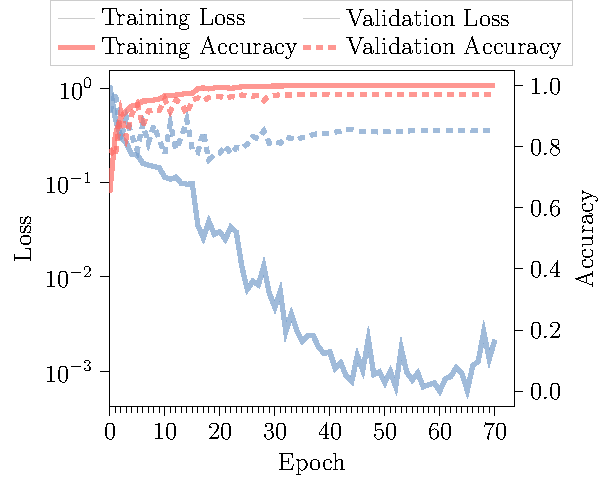
\includegraphics[width=\textwidth]{Figures/Appendix/DDSNet_2D.pdf}
    \caption{Model used in \gls{DDS}}\label{fig:DDSNet2D}
\end{subfigure}
\begin{subfigure}[t]{\modelplotwidth}
    \centering
    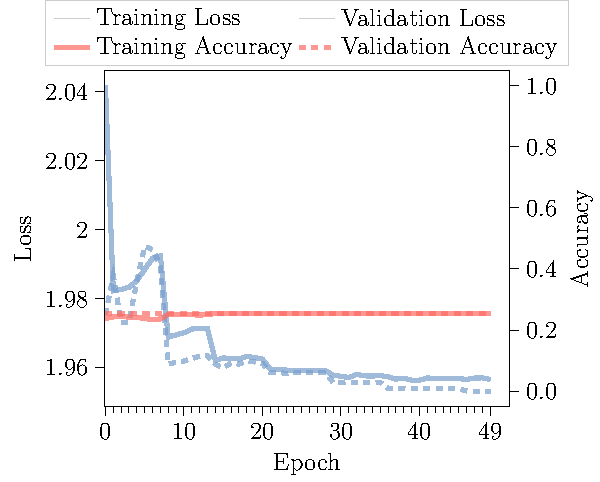
\includegraphics[width=\textwidth]{Figures/Appendix/AlexNet_2D.pdf}
    \caption{2D AlexNet}\label{fig:AlexNet2D}
\end{subfigure}
\begin{subfigure}[t]{\modelplotwidth}
    \centering
    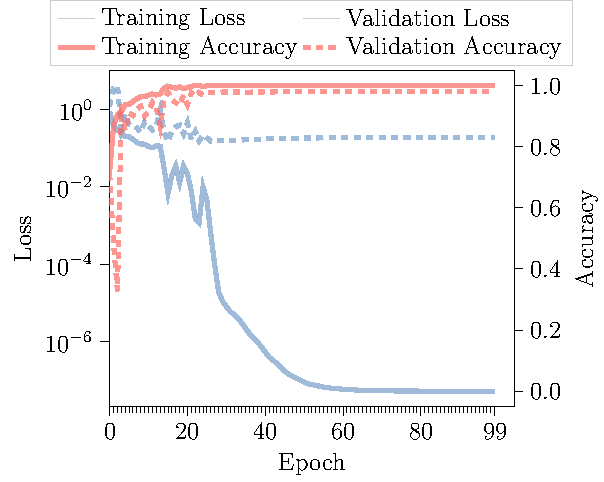
\includegraphics[width=\textwidth]{Figures/Appendix/DenseNet_2D.pdf}
    \caption{2D DenseNet121}\label{fig:DenseNet2D}
\end{subfigure}
\begin{subfigure}[t]{\modelplotwidth}
    \centering
    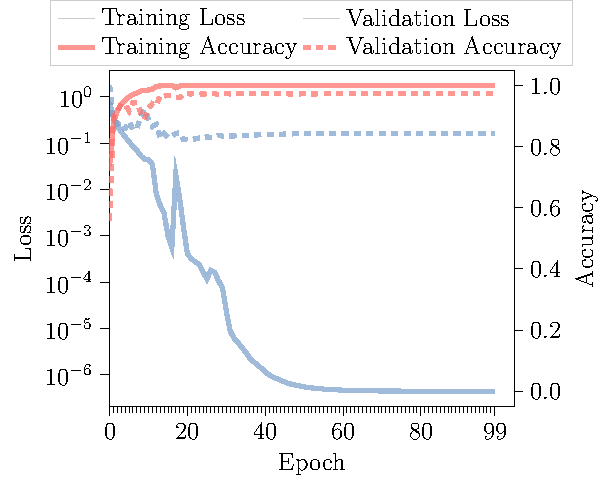
\includegraphics[width=\textwidth]{Figures/Appendix/ResNet_2D.pdf}
    \caption{2D ResNet18}\label{fig:ResNet2D}
\end{subfigure}

\begin{subfigure}[t]{\modelplotwidth}
    \centering
    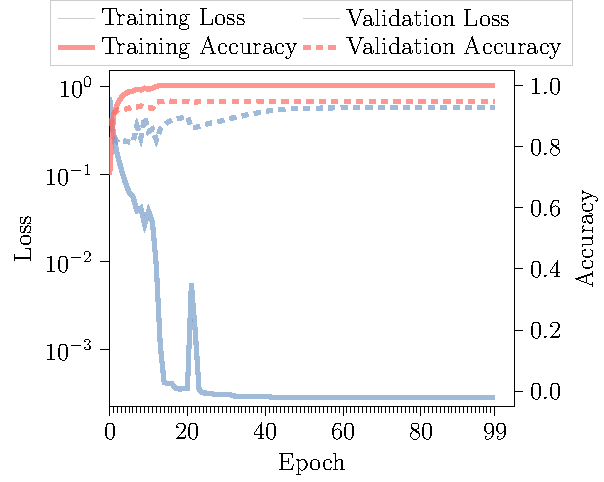
\includegraphics[width=\textwidth]{Figures/Appendix/VGG_2D.pdf}
    \caption{2D VGG19}\label{fig:VGG2D}
\end{subfigure}
\begin{subfigure}[t]{\modelplotwidth}
    \centering
    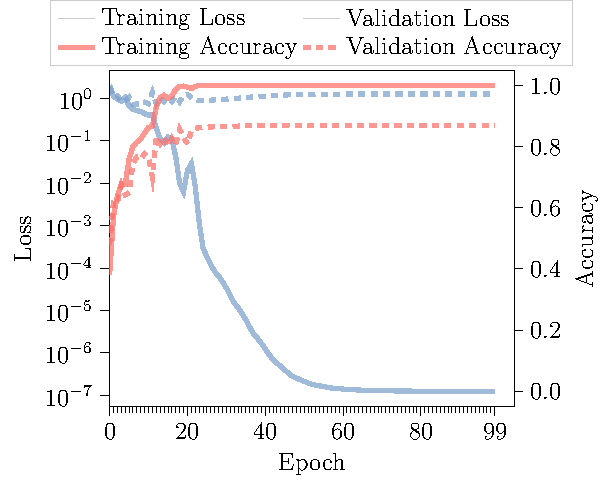
\includegraphics[width=\textwidth]{Figures/Appendix/DenseNet_3D.pdf}
    \caption{3D DenseNet121}\label{fig:DenseNet3D}
\end{subfigure}
\begin{subfigure}[t]{\modelplotwidth}
    \centering
    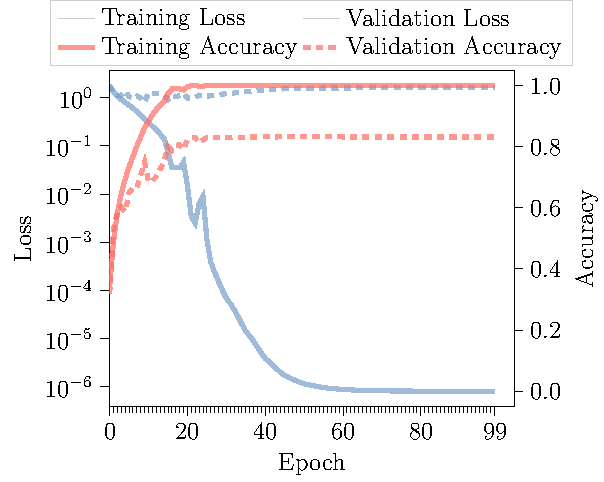
\includegraphics[width=\textwidth]{Figures/Appendix/ResNet_3D.pdf}
    \caption{3D ResNet18}\label{fig:ResNet3D}
\end{subfigure}

\caption{Learning curves of the different network architectures tested in the model parameter selection}\label{fig:modellearningcurves}
\end{sidewaysfigure}

\begin{table}[H]
 \centering
  \begin{tabular}{L{2.5cm}S[table-format=1.3]S[table-format=1.3]S[table-format=2.1]}
      \toprule
& {\textbf{Train}} & {\textbf{Validation}} & {\textbf{Training time (h)}}\\
    \midrule
    Our model & 0.999 & 0.971 & 14.8\\
    2D AlexNet & 0.255 & 0.255 & 11.0\\
    2D DensNet121 & 1.000 & 0.980 & 21.8\\
    2D ResNet18 & 1.000 & 0.973 & 26.4\\
    2D VGG19 & 1.000 & 0.948 & 34.6\\
    3D DenseNet121 & 1.000 & 0.868 & 22.9\\
    3D ResNet18 & 1.000 & 0.832 & 27.7\\
  \bottomrule
  \end{tabular}
  \caption{Overall training accuracy, overall validation accuracy, and the time it took to train each network for the different network architectures test in the model parameter selection.
  A train/validation split of the \gls{BTtrain} was used to determine the performance}\label{tab:modelaccuracies}

\end{table}

\clearpage

\section{Confusion matrices}
\label{app:confusionmatrices}

The confusion matrices for Experiment I (\cref{tab:seqresults}) and Experiment II (\cref{tab:confusion_adni}), which show the relation between the ground truth \gls{type} and the predicted \gls{type}.

{    % for making group where "\makegapedcells" is valid
\begin{table}[htbp]
\makegapedcells
% \hspace*{-2cm}
% \centering
\begin{tabular}{cc|cccccccc}
\multicolumn{2}{c}{}
            &   \multicolumn{8}{c}{\textbf{Predicted}} \\
    &       &   \rotatebox{-45}{\acrshort{T1}} & \rotatebox{-45}{\shortstack{\acrshort{T1C}}} & \rotatebox{-45}{\acrshort{T2}}  &  \rotatebox{-45}{\acrshort{PD}} & \rotatebox{-45}{\shortstack{T2w-\\FLAIR}}& \rotatebox{-45}{\acrshort{DWI}} & \rotatebox{-45}{\acrshort{DSC}} & \rotatebox{-45}{Derived}\\
    \cline{2-10}
\multirow{8}{*}{\rotatebox[origin=c]{90}{\textbf{Ground truth}\hspace{3cm}}}
    &\acrshort{T1}    & 433    & 2 & 0 & 1 & 0 &0 & 0 & 0\\[2ex]
    &\acrshort{T1C} & 2 & 608 & 0 & 0 & 0 & 0 & 0 & 0 \\[2ex]
    &\acrshort{T2} & 1    & 2    & 292   & 0     & 0     & 0     & 0   & 0\\[2ex]
    &\acrshort{PD} & 0    & 0    & 0     & 181   & 0     & 0     & 0   & 0 \\[2ex]
    &\acrshort{FLAIR}    & 18   & 0    & 0     & 0     & 238   & 0     & 0   & 0\\[2ex]
    &\acrshort{DWI}          & 0    & 0    & 0     & 0     & 0     & 344   & 2   & 1 \\[2ex]
    &\acrshort{DSC}      & 0    & 0    & 0     & 0     & 0     & 0     & 87 & 0 \\[2ex]
    &Derived      & 0    & 0    & 1     & 0     & 0     & 0     & 0   & 156\\[2ex]
    \cline{2-10}
    \end{tabular}
    \caption{Confusion matrix of results from Experiment I}\label{tab:seqresults}
\end{table}
 }

 {    % for making group where "\makegapedcells" is valid
\begin{table}[htbp]
\makegapedcells
% \hspace*{-2cm}
% \centering
\begin{tabular}{cc|cccccccc}
\multicolumn{2}{c}{}
            &   \multicolumn{8}{c}{\textbf{Predicted}} \\
    &       &   \rotatebox{-45}{\acrshort{T1}} & \rotatebox{-45}{\shortstack{\acrshort{T1C}}} & \rotatebox{-45}{\acrshort{T2}}  &  \rotatebox{-45}{\acrshort{PD}} & \rotatebox{-45}{\shortstack{T2w-\\FLAIR}}& \rotatebox{-45}{\acrshort{DWI}} & \rotatebox{-45}{\acrshort{DSC}} & \rotatebox{-45}{Derived}\\
    \cline{2-10}
    \multirow{8}{*}{\rotatebox[origin=c]{90}{\textbf{Ground truth}\hspace{3cm}}}
    &\acrshort{T1}        & 2655  & 1    & 0    & 0     & 0     & 0     & 0   & 0\\[2ex]
    &\acrshort{T1C}         & 0    & 0    & 0     & 0     & 0     & 0     & 0   & 0\\[2ex]
    &\acrshort{T2}          & 0    & 34   & 2140  & 44    & 0     & 0     & 0   & 0\\[2ex]
    &\acrshort{PD}          & 0    & 0    & 2     & 1067  & 0     & 0     & 0   & 0 \\[2ex]
    &\acrshort{FLAIR}    & 6    & 5    & 0     & 1     & 468   & 12    & 0   & 0\\[2ex]
    &\acrshort{DWI}          & 0    & 0    & 0     & 0     & 0     & 557   & 3   & 0 \\[2ex]
    &\acrshort{DSC}      & 0    & 0    & 0     & 0     & 0     & 0     & 0   & 0 \\[2ex]
    &Derived      & 0    & 0    & 1     & 0     & 0     & 3     & 0    & 228\\[2ex]
   \cline{2-10}
    \end{tabular}
    \caption{Confusion matrix of results from Experiment II}\label{tab:confusion_adni}
\end{table}

 }


\clearpage

\section{Predictive performance on per-\glsfmtlong{slice} basis}
\label{app:sliceresults}

\cref{tab:acc_slices} shows the accuracy of the \glspl{CNN} from Experiment I and Experiment II on a per-\gls{slice} basis instead of on a per-\gls{scan} basis.
These results are obtained by comparing the predicted \gls{class} of a \gls{slice} directly with the ground truth \gls{class} of that slice before the individual \gls{slice} predictions are combined by a majority vote to obtain the \gls{type}.

\begin{table}[ht]
 \centering
  \begin{tabular}{lS[table-format=1.3]S[table-format=1.3]}
      \toprule
& {\textbf{Experiment I}} & {\textbf{Experiment II}}\\
    \midrule
  Overall    & 0.934 & 0.851\\
  \cmidrule{2-3}
  \acrshort{T1}        & 0.942 & 0.814\\
  \acrshort{T1C}       & 0.940 & {\NA}\\
  \acrshort{T2}        & 0.926 & 0.894\\
  \acrshort{PD}        & 0.905 & 0.914\\
  \acrshort{FLAIR}  & 0.879 & 0.592\\
  \acrshort{DWI}        & 0.985 & 0.943\\
  \acrshort{DSC}    & 0.925 & {\NA}\\
  Derived    & 0.990 & 0.908\\
  \bottomrule
  \end{tabular}
  \caption{Overall accuracy and per-class accuracy achieved by \gls{DDS} in Experiment I and Experiment II on a per-\gls{slice} basis}\label{tab:acc_slices}

\end{table}

\clearpage
\section{Time comparison between \glsfmtlong{DDS}, \glsfmtlong{HC} and manual sorting}
\label{app:timing}

We estimated the potential time that can be saved by using \gls{DDS} to sort a \gls{ds} instead of doing so by hand or using \gls{HC}.
We did so by assuming the hypothetical situation where one has an automated tool that requires the \gls{T1C} and \gls{FLAIR} \glspl{scan} as inputs, and we compared the time needed to find the \gls{T1C} and \gls{FLAIR} \glspl{scan} for all \glspl{sub} and \glspl{ses} in the \gls{BTtest}.
The manual sorting was simulated by iterating over all \glspl{scan} in a \gls{ses} in random order until either the \gls{T1C} and \gls{FLAIR} \glspl{scan} were found or until there were no more \glspl{scan} to check.
The sorting of the \gls{ds} using \gls{HC} or \gls{DDS} was simulated by first iterating over all \glspl{scan} that were predicted as a \gls{T1C} or \gls{FLAIR} by these methods, and checking whether that prediction was correct.
If the predicted \gls{type} was incorrect, the same approach as for the manual sorting was followed to find the correct \glspl{scan}.
We assumed that, on average, a human required \num{25} seconds per \gls{scan} to visually identify the correct \gls{type}.
By multiplying this time per \gls{scan} with the total number of \glspl{scan} that were iterated over, we obtained an estimate for the total time taken by each method to find the \gls{T1C} and \gls{FLAIR} \glspl{scan}.
We used the \gls{BTtest} to evaluate the timing results, since \gls{HC} was only optimized for the \gls{BTset}.

\subsection{Results}
The time required to identify the \gls{T1C} and \gls{FLAIR} \gls{scan} for each \gls{ses} in the \gls{BTtest} by hand was estimated to be \num{29.0} hours.
The estimated time required to check and correct the automated \gls{type} recognition by \gls{HC} was \num{35.7} hours, which excludes the time required to construct the heuristic.
If the automated \gls{type} recognition was done by \gls{DDS} instead, we estimated that \num{12.3} hours of manual time were required.
The time required to run the \gls{DDS} pipeline on the \gls{ds} was \num{61.5} minutes using an Intel Xeon Processor E5-2690 v3 for pre-processing and post-processing, and an Nvidia Tesla K40m GPU to classify the \glspl{sample} using the \gls{CNN}.
If the \glspl{scan} identified by \gls{DDS} were used without a manual check, in which case the total sorting time was only \num{61.5} minutes, \num{527} \glspl{scan} would have been correctly identified.
Four \glspl{scan} were incorrectly identified as a \gls{T1C} or \gls{FLAIR} \gls{scan}, for one \gls{ses} the \gls{T1C} would not have been found, and for \num{8} \glspl{ses} the \gls{FLAIR} would not have been found.

It should be noted that with the automated methods (\gls{DDS} and \gls{HC}), one gets a fully sorted \gls{ds}, whereas the sorting by hand still requires the sorting of the \glspl{scan} that were not yet identified.

\clearpage

\section{Saliency map for full \glsfmtlong{scan}}
\label{app:saliency}

\cref{fig:saliency_lower_slices} and \cref{fig:saliency_upper_slices} show the saliency maps for all \num{25} \glspl{slice} from the \glspl{scan} of the example \gls{sub} from \cref{fig:seq_examples}.
The \gls{CNN} seems to focus on the same features as in \cref{fig:seq_gradcam}, mostly on the ventricles and on the \gls{CSF} at the edges of the brain.
In the superior \glspl{slice} of the \gls{scan}, it can be seen that the presence of a \gls{tumor} does not disrupt the \gls{CNN}.
Although it looks at the edge of the \gls{tumor}, it does not put a lot of focus on the \gls{tumor} itself.
For the most superior \glspl{slice} of \gls{T1}, \gls{T1C} and \gls{T2} it can be seen that when the brain is no longer present in the \gls{slice} the \gls{CNN} loses it focus and seems to look randomly throughout the \gls{slice}.

\begin{figure}[ht]
\includegraphics[width=\textwidth]{Figures/Appendix/attention_overview_slices_0_12.pdf}
\caption{Saliency maps for \glspl{slice} \num{1} through \num{13} of the \gls{sub} from \cref{fig:seq_examples}}
\label{fig:saliency_lower_slices}
\end{figure}

\begin{figure}[ht]
\includegraphics[width=\textwidth]{Figures/Appendix/attention_overview_slices_13_24.pdf}
\caption{Saliency maps for \glspl{slice} \num{14} through \num{25} of the \gls{sub} from \cref{fig:seq_examples}}
\label{fig:saliency_upper_slices}
\end{figure}


\clearpage

\section{Saliency maps for additional examples}
\label{app:artifactsaliency}

\subsection{Random samples from the \gls{BTtest}}
\label{app:randomtumorsample}

To show the robustness of our method to differences in \gls{scan} appearance, as well as to imaging artifacts, we have randomly selected \num{20} \glspl{slice} of each \gls{type} from the \gls{BTtest}.
All of these \glspl{slice} were then passed through the \gls{CNN}, and we determined the saliency maps along with the predicted \gls{class} of each \gls{slice}.
This is the prediction based on the \gls{slice} itself, and thus before the majority vote.
The saliency maps and predicted \glspl{type} are shown in \cref{fig:random_1} and \cref{fig:random_2}.
We have highlighted \glspl{slice} that contain imaging artifacts (\textcolor{red}{$\dagger$}), have a poor image quality (\textcolor{green}{$\dagger$}), and \glspl{sub} with a large head tilt  (\textcolor{cyan}{$\dagger$}).
These saliency maps show that the \gls{CNN} is quite robust to the presence of a \gls{tumor}, the presence of imaging artifacts, or poor image quality, in most cases the \gls{CNN} still predicts the correct \gls{type}.


\begin{figure}[ht]
    \centering
    \includegraphics[width=\textwidth]{Figures/Appendix/Random_saliency_1}

    \caption{Saliency maps and predicted \gls{type} of randomly drawn \glspl{sample} from the \gls{BTtest}}
    \label{fig:random_1}
\end{figure}

\begin{figure}[ht]
    \centering
    \includegraphics[width=\textwidth]{Figures/Appendix/Random_saliency_2}

    \caption{Saliency maps and predicted \gls{type} of randomly drawn \glspl{sample} from the \gls{BTtest}}
    \label{fig:random_2}
\end{figure}


\clearpage

\subsection{Random samples from \gls{NTTS}}
The same approach as in \cref{app:randomtumorsample} has been applied to show the saliency maps from random samples of the \gls{NTTS}.
In this case, the saliency maps were derived using the trained model from Experiment II instead of Experiment I.
Once again the saliency maps and the predicted \gls{type} are shown in \cref{fig:random_adni_1} and \cref{fig:random_adni_2}.
We have highlighted \glspl{slice} that contain imaging artifacts, including hippocampus \glspl{scan} with a limited field of view, (\textcolor{red}{$\dagger$}), have a poor image quality (\textcolor{green}{$\dagger$}), and \glspl{sub} with a large head tilt (\textcolor{cyan}{$\dagger$}).


\begin{figure}[ht]
    \centering
    \includegraphics[width=\textwidth]{Figures/Appendix/ADNI_random_saliency_1.pdf}

    \caption{Saliency maps and predicted \gls{type} of randomly drawn \glspl{sample} from the \gls{NTTS}}
    \label{fig:random_adni_1}
\end{figure}

\begin{figure}[ht]
    \centering
    \includegraphics[width=\textwidth]{Figures/Appendix/ADNI_random_saliency_2.pdf}

    \caption{Saliency maps and predicted \gls{type} of randomly drawn \glspl{sample} from the \gls{NTTS}}
    \label{fig:random_adni_2}
\end{figure}


\clearpage


\subsection{Robustness against bright noise}

To test the effect of potential bright spots in the \gls{scan}, we performed an experiment where random bright spots were introduced in the \glspl{slice} from \cref{fig:seq_examples}.
Within each \gls{slice} \per{0.5} of voxels were randomly chosen, and the intensity of these voxels was set to the maximum intensity of the \gls{slice}.
We then determined the saliency maps for these slices and the predicted \gls{type}, the results are shown in \cref{fig:bright_noise}.


These results show that our method is quite robust against bright spots in a \gls{scan}.
Only for the \gls{T1} and \gls{DSC} \glspl{scan} there were \glspl{slice} that were misclassified.
In the case of the \gls{T1} \gls{slice}, there were two out of five \glspl{slice} that were predicted to be \gls{T1C}.
This is most likely caused by the \gls{CNN} having learned that a \gls{T1} and \gls{T1C} \gls{scan} have a similar appearance in general, but that the \gls{T1C} \gls{scan} has brighter spots.
In two cases the \gls{DSC} \gls{slice} was misclassified as a \gls{DWI}.
Probably this is caused by the \gls{CNN} seeing the random brightness spots outside the skull as imaging artifacts, which often show up in \gls{DWI} \glspl{scan} and less so in \gls{DSC} \glspl{scan}.
Although the \gls{CNN} misclassified the \gls{T1} and \gls{DSC} \glspl{slice} in some cases, when bright spots were introduced on all \num{25} \glspl{slice} of the \gls{T1} and \gls{DSC} \glspl{scan} (randomly for each \gls{slice}) and then passed through the network, the \gls{CNN} still predicted the correct \gls{type} of the \gls{scan} after the majority vote.

\begin{figure}[ht]
    \centering
    \includegraphics[width=\textwidth]{Figures/Appendix/saliency_noise.pdf}
    \caption{Saliency maps and predicted \glspl{type} of the derived \glspl{slice} from \cref{fig:seq_examples} after randomly setting some pixels to the maximum intensity.
    Every time the \gls{slice} with the added noise is shown, followed by the saliency map and predicted \gls{type} for the same \gls{slice} in the row below}
    \label{fig:bright_noise}
\end{figure}



\clearpage

\section{Feature map visualizations}
\label{app:filtervis}

\cref{fig:filter_result_T1_1} through \cref{fig:filter_result_T1_6} show the feature maps of all filters of each convolutional layer for the \gls{T1} \gls{slice} shown in \cref{fig:seq_examples}.
It can be seen that some filters mainly identify the skull (for example, filter 1 from convolutional layer 1), whereas other filters seem to focus on specific structure (for example, filter 4 from convolutional layer 1, which seems to identify gray matter).

\foreach \layer in {1, 2, 3, 4, 5, 6}
{
    \begin{figure}[ht]
        \centering
        \includegraphics[width=\textwidth]{Figures/Appendix/Filters/T1_conv2d_\layer.pdf}
        \caption{Feature map visualizations of the trained \acrshort{CNN} from Experiment I. These visualization were obtained by passing a \gls{T1}~\gls{slice} through the network, and showing the results directly after convolutional layer \layer.
        The \gls{slice} is the same as the one shown in \cref{fig:seq_examples}}
        \label{fig:filter_result_T1_\layer}

    \end{figure}
}

\end{subappendices}
